\documentclass{scrbook}

%!TEX root = thesis.tex

% Set german to default language and load english as well
\usepackage[english,ngerman]{babel}

% Set UTF8 as input encoding
\usepackage[utf8]{inputenc}

% Set T1 as font encoding
\usepackage[T1]{fontenc}
% Load a slightly more modern font
\usepackage{lmodern}
% Use the symbol collection textcomp, which is needed by listings.
\usepackage{textcomp}
% Load a better font for monospace.
\usepackage{courier}
% Load package to configure header and footer
\usepackage{scrlayer-scrpage}

\usepackage{acronym}
\usepackage{setspace}
\setstretch{1.2}


\newcommand*{\secref}[1]{\hyperref[{#1}]{\ref*{#1} \nameref*{#1}}}
% Set some options regarding the document layout. See KOMA guide
\KOMAoptions{%
  paper=a4,
  fontsize=11.5pt,
  parskip=half,
  headings=normal,
  BCOR=1cm,
  headsepline,
  headsepline=0.5pt,
  DIV=13}

% do not align bottom of pages
\raggedbottom

% set style of captions
\setcapindent{24pt} % do not indent second line of captions
\setkomafont{caption}{\small}
\setkomafont{caption}{\vspace*{3mm}}
\setkomafont{captionlabel}{\textbf}
\setcapwidth[c]{1\textwidth}

% load extended tabulars used in the list of abbreviation
\usepackage{tabularx}

% load the color package and enable colored tables
\usepackage[table]{xcolor}

\usepackage{pdfpages}


% define new environment for zebra tables
\usepackage{colortbl}
\newcommand{\mainrowcolors}{\rowcolors{1}{white}{white}}
\newenvironment{zebratabular}{\mainrowcolors\begin{tabular}}{\end{tabular}}
\newcommand{\setrownumber}[1]{\global\rownum#1\relax}
%\newcommand{\headerrow}{\normalfont\sffamily\color{maincolor}\setrownumber1}
%\rowcolor{maincolor!50}

% add main color to section headers
\usepackage[outermarks,noindentafter,nobottomtitles]{titlesec}
\titleformat{\section}[hang]{\Large\sffamily\color{maincolor}}{\thetitle}{8pt}{\vspace{-2mm}}{}
\titleformat{\subsection}[hang]{\large\sffamily\color{maincolor}}{\thetitle}{8pt}{}
\titleformat{\subsubsection}[hang]{\normalfont\sffamily\color{maincolor}}{\thetitle}{8pt}{}
\titleformat{\paragraph}[hang]{\bfseries\sffamily\color{maincolor}}{\thetitle}{8pt}{}

%Etwas aufwendiger für die Kapitelüberschriften:
\titleformat{\chapter}[display]
{\huge\sffamily\color{maincolor}} 
{\color{maincolor!30}\fontsize{60pt}{40pt}\selectfont\thechapter}
{-0.2cm} %is vertical space in [display] mode
{\vspace{-2mm}} %1ex ist die Hähe von x im aktuellen Font
[\vspace{-4mm}]

% do not print numbers next to each formula
\usepackage{mathtools}
\mathtoolsset{showonlyrefs}
% left align formulas
\makeatletter
\@fleqntrue\let\mathindent\@mathmargin \@mathmargin=\leftmargini
\makeatother

% Allow page breaks in align environments
\allowdisplaybreaks

% header and footer
\pagestyle{scrheadings}
\setkomafont{pagenumber}{\normalfont\sffamily\color{maincolor}}
\setkomafont{pageheadfoot}{\normalfont\sffamily}
\setkomafont{headsepline}{\color{maincolor}}

% German guillemets quotes
\usepackage[german=guillemets]{csquotes}

% load TikZ to draw diagrams
\usepackage{tikz}

% load additional libraries for TikZ
\usetikzlibrary{%
  automata,%
  positioning,%
}

% set some default options for TikZ -- in this case for automata
\tikzset{
  every state/.style={
      draw=maincolor,
      thick,
      fill=maincolor!18,
      minimum size=0pt
    }
}

% load listings package to typeset sourcecode
\usepackage{listings}

% set some options for the listings package
\lstset{%
  upquote=true,%
  showstringspaces=false,%
  captionpos=b,%
  basicstyle=\ttfamily,%
  keywordstyle=\color{keywordcolor}\slshape,%
  commentstyle=\color{commentcolor}\itshape,%
  stringstyle=\color{stringcolor}}
\renewcommand{\lstlistingname}{Quelltext}
\renewcommand{\lstlistlistingname}{Quelltextverzeichnis}

% enable german umlauts in listings
\lstset{
literate={ö}{{\"o}}1
{Ö}{{\"O}}1
{ä}{{\"a}}1
{Ä}{{\"A}}1
{ü}{{\"u}}1
{Ü}{{\"U}}1
{ß}{{\ss}}1
}

% define style for pseudo code
\lstdefinestyle{pseudo}{language={},%
  basicstyle=\normalfont,%
  morecomment=[l]{//},%
  morekeywords={for,to,while,do,if,then,else},%
  mathescape=true,%
  columns=fullflexible}

% load the AMS math library to typeset formulas
\usepackage{amsmath}
\usepackage{amsthm}
\usepackage{thmtools}
\usepackage{amssymb}

% load the paralist library to use compactitem and compactenum environment
\usepackage{paralist}

% load varioref and hyperref to create nicer references using vref
\usepackage[ngerman]{varioref}
\PassOptionsToPackage{hyphens}{url} % allow line break at hyphens in URLs
\usepackage{hyperref}

% setup hyperref
\hypersetup{breaklinks=true,
  pdfborder={0 0 0},
  ngerman,
  pdfhighlight={/N},
  pdfdisplaydoctitle=true}

% Fix bugs in some package, e.g. listings and hyperref
\usepackage{scrhack}

% set the style of the bibliography
\usepackage{apacite}
\bibliographystyle{apacite}

% Allow todos
\usepackage{todonotes}

% define german names for referenced elements
% (vref automatically inserts these names in front of the references)
\labelformat{figure}{Abbildung\ #1}
\labelformat{table}{Tabelle\ #1}
\labelformat{appendix}{Anhang\ #1}
\labelformat{chapter}{Kapitel\ #1}
\labelformat{section}{Abschnitt\ #1}
\labelformat{subsection}{Unterabschnitt\ #1}
\labelformat{subsubsection}{Unterunterabschnitt\ #1}
\AtBeginDocument{\labelformat{lstlisting}{Quelltext\ #1}}

% define theorem environments
\declaretheorem[numberwithin=chapter,style=plain]{Theorem}
\labelformat{Theorem}{Theorem\ #1}

\declaretheorem[sibling=Theorem,style=plain]{Lemma}
\labelformat{Lemma}{Lemma\ #1}

\declaretheorem[sibling=Theorem,style=plain]{Korollar}
\labelformat{Korollar}{Korollar\ #1}

\declaretheorem[sibling=Theorem,style=definition]{Definition}
\labelformat{Definition}{Definition\ #1}

\declaretheorem[sibling=Theorem,style=definition]{Beispiel}
\labelformat{Beispiel}{Beispiel\ #1}

\declaretheorem[sibling=Theorem,style=definition]{Bemerkung}
\labelformat{Bemerkung}{Bemerkung\ #1}

%!TEX root = thesis.tex

% Use this file to define some macros you need in your thesis. A macro is a short command that inserts some mathematical symbols or texts you do not want to retype each time you need some. I recommend to use as many macros as possible, because you are able to change them later. For example if you use the same macro each time you need to give the formal semantics of an expression you can easily change the appearance of these brackets by updating the macro later on.

% Set of natural numbers
\newcommand{\N}{\mathbb{N}}

% The default epsilon does not look very nice
\let\epsilon\varepsilon

% If you need to use mathematical expressins like an epsilon in the section titles of your thesis you will end up with warnings that these special symbols cannot be included in the PDF favorites. The following macro uses the mathematical symbol during the text of the thesis and the string "Epsilon" in the PDF favorites.
\newcommand{\pdfepsilon}{\texorpdfstring{$\epsilon$}{Epsilon}}


% Set title and author used in the PDF meta data
\hypersetup{
  pdftitle={Snipe-IT Companion: Entwicklung eines Reservierungstools für Assets},
  pdfauthor={Anna-Tabea Manske}
}

% Depending on which of the following two color schemes you import your thesis will be in color or grayscale. I recommend to generate a colored version as a PDF and a grayscale version for printing.

%!TEX root = thesis.tex

% define color of example university
\xdefinecolor{exampleuniversity}{RGB}{0,62,75}


\colorlet{maincolor}{exampleuniversity}
%\colorlet{maincolor}{mycolor}

\colorlet{stringcolor}{green!60!black}
\colorlet{commentcolor}{maincolor!30}
\colorlet{keywordcolor}{maincolor!80!black}

\newcommand{\imagesuffix}{-color}
%%!TEX root = thesis.tex

\colorlet{maincolor}{black}

\colorlet{stringcolor}{black}
\colorlet{commentcolor}{black!50}
\colorlet{keywordcolor}{black}

\newcommand{\imagesuffix}{-gray}

\newcommand{\duedate}{03. Novemeber 2022}

\begin{document}
\frontmatter
%!TEX root = thesis.tex

\begin{titlepage}
  \centering
  \thispagestyle{empty}

  \vskip1cm

  \pgfimage[height=2.5cm]{Bilder/uni-logo-example\imagesuffix}

  \vskip2.5cm

  \LARGE

  \textbf{\sffamily\color{maincolor}Snipe-IT Companion: Entwicklung eines Reservierungstools für Assets}

  {\sffamily Snipe-IT Companion: Development of a Reservation Tool for Assets}

  \normalfont\normalsize

  \vskip2em

  \textbf{\sffamily\color{maincolor}Bachelorarbeit}

  im Rahmen des Studiengangs \\
  \textbf{\sffamily\color{maincolor}Medieninformatik} \\
  der Universität zu Lübeck

  \vskip1em

  vorgelegt von \\
  \textbf{\sffamily\color{maincolor}Anna-Tabea Manske}

  \vskip1em

  ausgegeben und betreut von \\
  \textbf{\sffamily\color{maincolor} Univ.-Prof. Dr. rer. nat. Hans-Christian Jetter}

  \vskip1em

  mit Unterstützung von\\
  Jan-Henrik Schröder, M.Sc.

  \vskip1em


  \vfill

  Lübeck, den \duedate
\end{titlepage}



%!TEX root = thesis.tex

\cleardoublepage
\thispagestyle{plain}

\pdfbookmark{Kurzfassung}{kurzfassung}
\section*{Kurzfassung}
\todo{Neu: bitte rüberlesen}
Am \ac{imis} werden Assets ohne Anmeldung oder nur mit einer mündlichen Absprache verwendet. Für die
vorausschauende Planung von anstehenden Projekten gibt es keine feste Reservierung oder einen
Überblick, wann die gewünschten Assets wieder verfügbar sind. Zudem ist vielen Mitarbeitenden und
Studierenden der Universität zu Lübeck unklar, welche Assets sich in den Laboren des \ac{imis}
befinden.

Das Ziel der vorliegenden Arbeit ist die Entwicklung eines wirksamen Systems, welches den
Reservierungs- und Ausleihprozess am \ac{imis} einheitlicher, effizienter und zufriedenstellender
lösen lässt. Die Basis für das Reservierungstool schafft die Asset-Managementsoftware
\textit{Snipe-IT}, welche bereits am \ac{imis} eingesetzt wurde.

Aus diesem Grund wurde in der vorliegenden Arbeit den Forschungsfragen nachgegangen, welche zentrale
Schwierigkeiten die aktuelle Planung und Reservierung von Assets für Mitarbeitende und Studierende
mit sich bringt und welche Anforderungen ein System mitbringen sollte, um diese zu adressieren und
reduzieren. Dazu wurden in der vorliegenden Arbeit systematische und standardisierte Anforderungen
an ein solches Reservierungstool auf Basis von Nutzenden, Aufgaben und Kontexten entwickelt und in
einer formalisierten Anforderungsanalyse erfasst. Teile des Konzeptes wurden in Form eines
technologisch reifen Prototyps realisiert. Die Ergebnisse der Evaluation zeigten, dass das System
als Unterstützung wahrgenommen wurde. Aufseiten der Ausleihenden wurden alle Funktionalitäten
überwiegend als hilfreich eingestuft. Auch aus Sicht der Verleihenden war die Nutzung des Systems
überwiegend positiv eingestuft worden.  Da das positive Ergebnis der durchgeführten Studie nicht mit
einem weiteren System verglichen werden konnte, wurde eine weitere ausführlichere Studie mit einem
Vergleichsystem empfohlen. Abschließend wurde die Weiterentwicklung des Systems und Folgestudien zur
Evaluation der Anwendung vorgeschlagen und diskutiert.

\subsection*{Schlüsselwörter}
Mensch-Computer-Interaktion, Reservieren, Assetmanagement, Snipe-IT, Dashboard, Web-App, Framework

\cleardoublepage
\thispagestyle{plain}

\foreignlanguage{english}{%
  \pdfbookmark{Abstract}{abstract}
  \section*{Abstract} 


  \subsection*{Keywords}
  Human-Computer Interaction, Reservation, Asset Management, Snipe-IT, Dashboard, Web App, Framework

  }

\cleardoublepage
\phantomsection
\pdfbookmark{\contentsname}{tableofcontents}
\markboth{\contentsname}{}
\tableofcontents

\mainmatter
%!TEX root = thesis.tex

\chapter{Einleitung}
Das Ausleihen von Assets jeglicher Art ist keine Neuheit \cite{soderholm2018borrowing}. An der
Zentralen Hochschulbibliothek Lübeck (ZHB) wird hierzu beispielsweise die Buchungsapp
\textit{Affluences}\footnote{\url{https://affluences.com/?lang=de}} verwendet. Zum Ausleihen von
Materialien müssen Terminabholungen online gebucht werden \cite{zhb_offnung_nodate}. Die Anfragen
können überprüft werden, wodurch das vorausschauende Planen der Materialien ermöglicht wird. 

Am Institut für Multimediale und Interaktive Systeme (\ac{imis}) werden Assets ohne Anmeldung oder
mit einer mündlichen Absprache verwendet. Aufseiten der Mitarbeitenden wird der Gebrauch der Assets
individuell geplant, sodass das frühzeitige Reservieren oder das geplante Ausleihen erschwert wird.
Für die vorausschauende Planung von anstehenden Projekten gibt es keine feste Reservierung oder
einen Überblick, wann die gewünschten Assets wieder verfügbar sind. Zudem ist vielen Mitarbeitenden
unklar, welche Assets sich in den Laboren des \ac{imis} befinden. Folglich kennen Mitarbeitende nur
selten die Möglichkeiten, mit denen sie ihre Forschungsprojekte oder die Lehre ergänzen könnten.

\todo{Neu: Kommender Absatz überarbeitet}
Aktuell werden Reservierungen sowie der Gebrauch von Equipment über unterschiedliche
Kommunikationswege, wie E-Mail oder mündlicher Absprache bei zuständigen Mitarbeitenden angefragt.
Die zuständigen Mitarbeitenden prüfen die Anfrage und koordinieren potenzielle Kollisionen mit
bereits reservierten Zeiträumen oder Absprachen und bestätigen, ändern oder lehnen diese
(Reservierungs-)Anfrage ab. In einigen Fällen werden die gebuchten Zeiten auf Papier dokumentiert.
Aufseiten der Studierenden kann ein Reservierungstool für Projekte, wie zum Beispiel die des Moduls
\ac{emi} hilfreich sein. Studierende müssen während dieses Projekts eine multimediale Abgabe
produzieren, welche beispielsweise die Form eines Videos haben kann.\\ Aktuell ist vielen
Studierenden nicht bewusst, dass das \ac{imis} Equipment wie Kameras, Gimbals oder VR-Equipment für
Videos oder Projektaufgaben bereitstellt. Des Weiteren sind Hemmschwelle und Aufwand zum Ausleihen
der Hardware hoch, da uneindeutig ist, welche Mitarbeitenden für die jeweilige Hardware zuständig
sind.

\section{Ziel der Arbeit}
Das Ziel dieser Arbeit ist es ein wirksames System zu entwickeln, welches den Reservierungs- und
Ausleihprozess am \ac{imis} einheitlicher, effizienter und zufriedenstellender lösen lässt. Die
Anwendung soll es unter anderem ermöglichen, die auszuleihenden Assets in einer Liste abzubilden und
diese zu durchsuchen. In diesem Zusammenhang soll auch das Anzeigen einer Stückzahl der jeweils
verfügbaren Assets, deren Bedienungsanleitung sowie die verantwortlichen Mitarbeitenden umgesetzt
werden. Das Reservierungstool soll eine niedrigschwellige Möglichkeit bieten, um Mitarbeitenden die
Arbeit im Reservierungsprozess zu erleichtern. Außerdem soll es eine Übersicht über Assets
geben, sodass Mitarbeitende nicht mehr im Unklaren über die Hardware-Möglichkeiten sind und das
Material optimal genutzt werden kann.

Die Basis für ein solches Tool schafft die Asset-Managementsoftware \textit{Snipe-IT}
\cite{noauthor_home_nodate}, welche bereits am \ac{imis} eingesetzt wird. \textit{Snipe-IT} ist eine
kostenlose, quelloffene IT-Asset-Verwaltungs-Plattform, welche das Nachverfolgen von
Software-Lizenzen, Hardware und Verbrauchsgegenständen ermöglicht. Genannte Assets können über ein
Dashboard hinzugefügt, verwaltet und gelöscht werden. Über Labels können Assets zur
Übersichtlichkeit in verschiedene Kategorien eingeordnet werden, während Tags ein Asset eindeutig
identifizieren (z. B. Seriennummer). Zudem ermöglicht das „Checkin/Checkout“-System die
Nachverfolgung aller Assets, falls diese zum Beispiel an eine Person ausgeliehen werden. Zu jedem
Zeitpunkt kann ein Asset maximal einer Person zugeordnet werden, wodurch das mehrfache gleichzeitige
Ausleihen eines Assets verhindert wird. Da \textit{Snipe-IT} selbst die zukünftige Reservierung
nicht unterstützt, umfasst das Ziel der Arbeit einen \textit{Snipe-IT Companion}, welcher das
Ausleihen in die Zukunft möglich macht.


\section{Forschungsfragen}
\label{sec:Forschungsfragen}
Im Sinne der eingangs beschriebenen Ziele soll im Rahmen der vorliegenden Arbeit untersucht werden,
wie ein Reservierungstool gestaltet werden kann, um Mitarbeitende und Studierende darin zu
unterstützen, Assets einzusehen und ausleihen zu können.

Um den aktuellen Stand und die Probleme des aktuellen Ausleihprozess nachvollziehen zu können,
müssen diese zunächst ermittelt und klassifiziert werden. Die erste Forschungsfrage beschäftigt sich
daher mit der Analyse der Schwierigkeit des Ausleihprozesses.
\begin{enumerate}
  \item[\sffamily\color{maincolor} {F1 |}] {Welche zentralen Schwierigkeiten bringt die aktuelle Planung und Reservierung von Assets für Mitarbeitende und Studierende mit sich?}
\end{enumerate}
Um die zentralen Schwierigkeiten und Probleme lösen zu können, müssen Anforderungen an das System
ermittelt werden. Anschließend müssen diese nach Relevanz sortiert werden, um möglichst viele
Schwierigkeiten lösen zu können. Die zweite Forschungsfrage beschäftigt sich folglich mit den
Anforderungen, welche ein solches Reservierungstool umfassen sollte, um die Schwierigkeiten zu minimieren.
\begin{enumerate}
  \item[\sffamily\color{maincolor} {F2 |}] {Was sind Anforderungen an ein System, welches die in F1 gezeigten Schwierigkeiten adressiert und reduziert?}
\end{enumerate}
Abschließend soll eruiert werden, ob die erste Iteration des Systems die ermittelten Schwierigkeiten
mit den erarbeiteten Funktionalitäten lösen kann. Die letzte Forschungsfrage beschäftigt sich
demzufolge mit der Evaluation des erarbeiteten Systems und den möglichen Stärken und Schwächen.
\begin{enumerate}
  \item[\sffamily\color{maincolor} {F3 |}] {Inwieweit kann ein aus F2 resultierender Prototyp die in F1 identifizierten Schwierigkeiten reduzieren?}
\end{enumerate}

\section{Vorgehensweise}
Die Entwicklung des Systems orientiert sich am menschenzentrierten Gestaltungsprozess
\cite{DINISO9241}. Der Prozess teilt sich im Rahmen dieser Arbeit in
fünf aufeinanderfolgende Phasen (\ref{fig:vorgehen}), wobei die Entwurfs- und Implementierungsphasen
Spielraum für ein iteratives Vorgehen lassen. Unter anderem werden in der Analyse die Aufgaben des
Systems, die Nutzenden und der Kontext nach dem Entwicklungsprozess für interaktive Medien
aufgeführt, um ein gebrauchstaugliches Ergebnis erzielen zu können \cite{HerczegMDI2009}.

\begin{figure}[h]
  \centering
  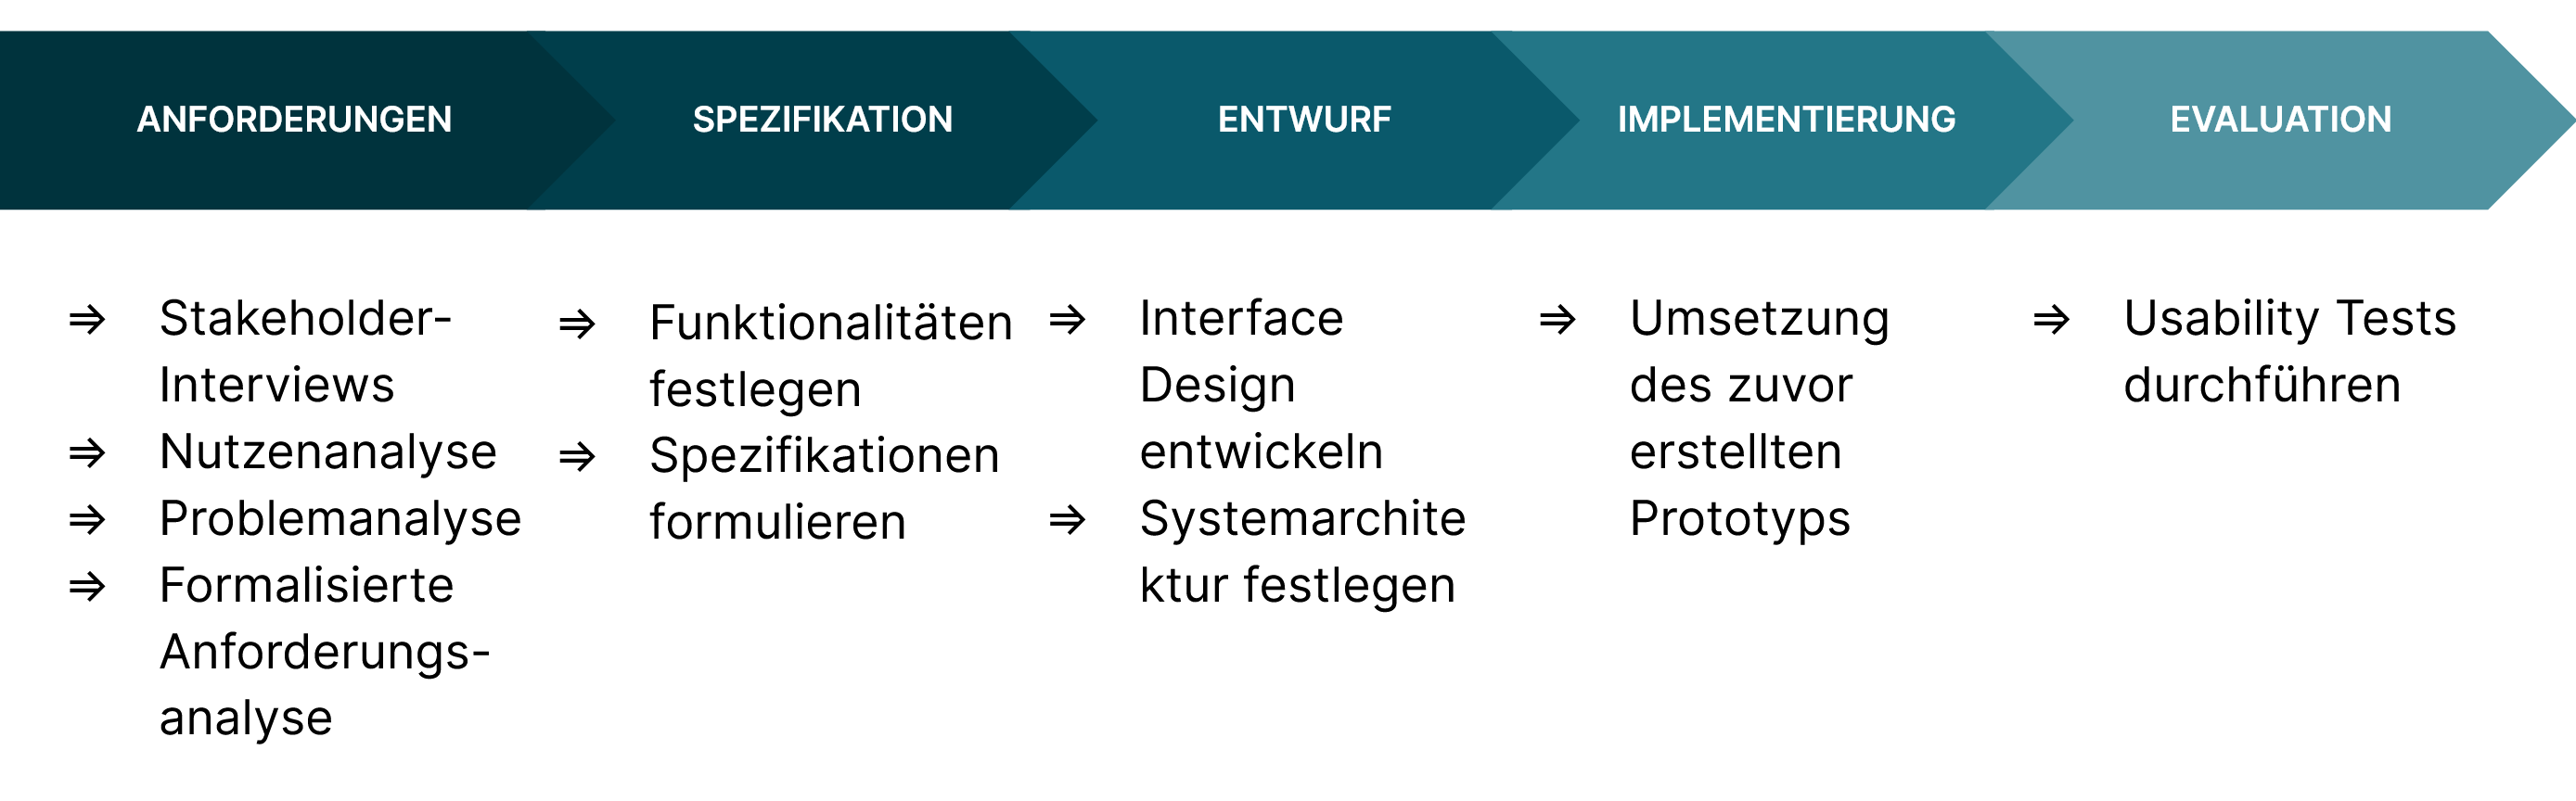
\includegraphics[scale=0.156]{Bilder/vorgehen.png}
  \label{fig:vorgehen}
  \caption[Vorgehensmodell]{Vorgehensmodell}
\end{figure}

In der ersten Phase werden die Anforderungen an das zu entwickelnde System erarbeitet und
verstanden. Die Erkenntnisse dieser Phase sind in \ref{chapter-analyse} zu finden.
\ref{chapter-analyse} soll unter anderem die Forschungsfragen F1 und F2 beantworten. Durch
semi-strukturierte Interviews mit Stakeholdern sollen die zentralen Schwierigkeiten und Aufgaben des
Ausleihprozesses festgestellt werden. Folglich werden die Notwendigkeit der angedachten
Anforderungen mithilfe der Interviews überprüft und ergänzt. Außerdem wurde eine Recherchiere
vergleichbarer Systeme durchgeführt, um die Aussagekraft der ermittelten Interviewergebnisse zu
überprüfen.

\todo{Neu: Kommender Absatz überarbeitet}
In der Spezifikationsphase werden die Anforderungen an das System weiter spezialisiert
(\ref{chapter-konzept}). Daher werden Funktionalitäten entsprechend den Anforderungen entwickelt und
in einer priorisierten Feature-Liste festgehalten. Anschließend wird die Systemarchitektur,
aufgeteilt in Frontend, Reservierungsinterface (Backend) und dem bestehenden Snipe-IT Server,
mithilfe des C4-Models erarbeitet. Aufbauend darauf werden passende Frameworks zur Entwicklung
ausgewählt. Darüber hinaus wird das Interface-Design erarbeitet (\ref{chapter-design}). Hierbei wird
durch Usability Tests ein iteratives Vorgehen ermöglicht.
 

Die Implementierungsphase umfasst die eigentliche Umsetzung des Reservierungstools
(\ref{chapter-implementierung}). Hierbei werden die in der Konzeptionsphase festgelegten Frameworks
genutzt. \ref{chapter-dialogbeispiel} präsentiert das realisierte System anhand von
Dialogbeispielen.

In der abschließenden Phase wird das realisierte System mithilfe von Interviews und Umfragen
evaluiert (\ref{chapter-evaluation}). Die Ergebnisse der Phase beantworten Forschungsfrage F3 und
geben Aufschluss über die Wirksamkeit des entwickelten Systems. Im Anschluss gibt
\ref{chapter-fazit} einige Perspektiven über offene Punkte und die mögliche Weiterentwicklung des
Systems.
\chapter{Anforderungen}
\label{chapter-analyse}

Um Benutzende, Aufgaben und Kontext des Projektes genauer zu verstehen, wurde eine Analyse nach dem
menschenzentrierten Gestaltungsprozess durchgeführt \cite{DINISO9241}.
Hierbei wurden relevante Anforderungen, die Einfluss auf die Entwicklung und die spätere Nutzung des
Reservierungstools nehmen, identifiziert und eingeordnet. Mit der Durchführung einer Recherche,
welche in den Datenquellen (\ref{section:daten}) genauer präsentiert wird, wurden zunächst zwei
Benutzergruppen (Verleihende und Ausleihende) festgehalten. Mittels einer Benutzeranalyse
(\ref{section:benutzer}) unter der Zuhilfenahme von durchgeführten Interviews, konnten diese weiter
klassifiziert und eingegrenzt werden. Daraufhin wurden die Probleme und Herausforderungen des
aktuellen Vorgehens und den unterschiedlichen Ausleihprozessen (\ref{section:iststand}) hergeleitet.
Anschließend wurden die Aufgaben, die Verleihende und Ausleihende mithilfe der Anwendung bewältigen
sollten, diskutiert (\ref{section:aufgaben}). Abschließend wurde der organisatorische und
zeitlich-räumliche Kontext des Verleihens und Ausleihens am \ac{imis} (\ref{section:kontext})
untersucht. Aufbauend auf den Resultaten der vorangestellten Untersuchungen wurden die objektiven
Anforderungen an den Snipe-IT Companion nach \citeA{Balzert2009} formalisiert
(\ref{section:anforderung}). Diese dienen als Grundlage für das gesamte Konzept der Arbeit.

\section{Datenquellen}
\label{section:daten}
Im Rahmen der Analyse wurden \nameref{subsection:interview} durchgeführt
(\ref{subsection:interview}). Darauffolgend wurde nach vergleichbaren Projekten und Systemen
recherchiert (\ref{subsection:system}).

\subsection{Stakeholder-Interviews}
\label{subsection:interview}
\todo[inline]{bei denen es um die subjektive Sicht von Personen geht, die unterschiedlich ausfallen und
begründet werden können – hier liegt eine Stärke qualitativer Verfahren, weil sie z.B. in Interviews
dem Befragten für eigene Sinngebungen, Deutungen etc. Raum geben (vgl. Bortz  Döring 2016, 184.}

Zunächst wurde anhand der zu untersuchenden Gesichtspunkte ein Interviewleitfaden für ein
semi-strukturiertes Interview entwickelt (\ref{appendix:interview}). Mithilfe dieses Leitfadens
wurden die Befragten durch das Interview geführt. Die Interviews wurden aufgezeichnet und
anschließend in Teilen, mithilfe eines vereinfachten Transkriptionssystems, verschriftlicht
\cite{dresing_praxisbuch_2016}. Daraufhin wurde eine qualitative Inhaltsanalyse durchgeführt.
Hierfür wurden die Transkripte erneut gelesen und für die Arbeit und Forschungsfragen relevante
Textstellen kommentiert. Infolgedessen wurden die erarbeiteten Kommentare in ein Ordnungssystem
strukturiert und unter den einzelnen Analysepunkten zusammengefasst \cite{dresing_praxisbuch_2016}.

Es wurde eine Unterteilung in Verleihende und Ausleihende von Assets vorgenommen (genauere
Definition der Benutzergruppen in \ref{section:benutzer}). Bei den Teilnehmenden handelt es sich um
Mitarbeitende, welche am \ac{imis} tätig sind und Studierende der Medieninformatik an der
Universität zu Lübeck. In \ref{table:v} ist der jeweilige (Haupt-)Zuständigkeitsbereich der
Verleihenden aufgeführt. Verleihende der Assets können gleichzeitig die Position eines Ausleihenden
einnehmen. Die Ausleihenden umfassen außerdem Studierende, welche in \ref{table:a} dargestellt sind.
Durch den geplanten Einsatz am \ac{imis} wurde sich zunächst ausschließlich auf \ac{wimi} des
\ac{imis} und Studierende der Medieninformatik begrenzt. Hierbei wurde insbesondere der Fokus auf
die Probleme am \ac{imis} gelegt (genauere Untersuchungen in der Problemanalyse in
\ref{section:iststand}). Die IDs der Teilnehmenden werden als Verweise in den folgenden Abschnitten
verwendet.

\begin{table}[h]
        \centering
        \caption{Teilnehmende der Interviews, Verleihende}
        \begin{tabular}{lll}
                \arrayrulecolor{maincolor}\hline
                \sffamily\color{maincolor}ID & \sffamily\color{maincolor}Alter &
                \sffamily\color{maincolor}Zuständigkeitsbereich                                   \\
                \arrayrulecolor{maincolor}\hline
                V1                           & 25 - 35 J.                      & Keine direkte
                Zuständigkeit, Zugänge zu verschiedenen Laboren                                   \\
                V2                           & 25 - 35 J.                      & Multimedialabor
                \\
                V3                           & 25 - 35 J.                      & VR-Labor
                \\
                V4                           & 40 - 59 J.                      & Administratives
                Personal                                                                          \\
                V5                           & 25 - 35 J.                      & Innovationslabor
                \\
                \arrayrulecolor{maincolor}\hline
        \end{tabular}
        \label{table:v}
\end{table}

\begin{table}[h]
        \centering
        \caption{Teilnehmende der Interviews, Ausleihende \\
                (die mit * gekennzeichneten Personen wurden gemeinsam interviewt)}
        \begin{tabular}{lll}
                \arrayrulecolor{maincolor}\hline
                \sffamily\color{maincolor}ID & \sffamily\color{maincolor}Alter &
                \sffamily\color{maincolor}Rolle                                                     \\
                \arrayrulecolor{maincolor}\hline
                A1                           & 19 - 25 J.                      & Bachelorstudentin,
                Hilfswissenschaftlerin                                                              \\
                A2                           & 19 - 25 J.                      & Bachelorstudent
                \\
                A3                           & 19 - 25 J.                      & Masterstudent,
                Hilfswissenschaftler                                                                \\
                A4*                          & 19 - 25 J.                      & Bachelorstudentin
                \\
                A5*                          & 19 - 25 J.                      & Bachelorstudentin
                \\
                A6                           & 19 - 25 J.                      & Masterstudentin
                \\
                \arrayrulecolor{maincolor}\hline
        \end{tabular}
        \label{table:a}
\end{table}

Des Weiteren wurde mithilfe des \ac{ati} das technische Interesse und Verständnis der Teilnehmenden
festgestellt (\ref{table:ati}) \cite{attig_assessing_2017}. In beiden Gruppen konnten lediglich
geringe Unterschiede innerhalb der soziodemografischen Daten festgestellt werden. Neben diesen Daten
ist im Kontext der vorliegenden Arbeit insbesondere die Technikaffinität relevant. 

Insgesamt konnte für beide Gruppen eine Einschätzung der Technikaffinität anhand der \ac{ati}-Skala
ermittelt werden (Verleihende: M=5.00, SD=0.58, N=3; Ausleihende: M=5.09, SD=0.48, N=9)
(\ref{table:ati}). Durch das Heranziehen zweier Vergleichsstichproben aus
\citeA{franke_personal_2019} (M=4.14, N=300 und M=4.23, N=65), lässt sich schlussfolgern, dass die
Nutzendengruppen eine vergleichsweise hohe Technikaffinität ausweisen.



\begin{table}[h]
        \centering
        \caption{Ergebniswerte der \ac{ati}-Skala}
        \begin{tabular}{lccc}
                \arrayrulecolor{maincolor}\hline
                \sffamily\color{maincolor}Benutzergruppe & \sffamily\color{maincolor}Mittelwert
                $(M)$                                    & \sffamily\color{maincolor}Standardabweichung $(SD)$ &
                \sffamily\color{maincolor}Teilnehmende $(N)$                                                          \\
                \arrayrulecolor{maincolor}\hline
                Verleihende                              & 5.00                                                & 0.58
                                                         & 3                                                          \\
                Ausleihende                              & 5.09                                                & 0.48
                                                         & 9                                                          \\
                \arrayrulecolor{maincolor}\hline
        \end{tabular}
        \label{table:ati}
\end{table}

\subsection{Recherche vergleichbare Systeme}
\label{subsection:system}
Für die Recherche wurden die digitalen Bibliotheken ACM Digital
Library\footnote{\url{https://dl.acm.org/}} und Google
Scholar\footnote{\url{https://scholar.google.de/}} genutzt. Es wurden Begriffe aus den Bereichen
Managementsystem \textit{(Assets, Assetmanagement, schedule)} und Reservation \textit{(reservation,
Lending, lend, borrow)} zur Suche verwendet. Die Recherche sollte dem besseren Vergleichen und
Abwägen der analysierten Interview-Ergebnisse dienen und vergleichbare Systeme und Projekte
eruieren. Des Weiteren sollte die Recherche dazu dienen mögliche Fehlerquellen zu erörtern, um diese
umgehen zu können. Durch den speziellen Einsatzort am \ac{imis} stellte sich zeitnah heraus, dass
wenige bis keine vergleichbaren Systeme gefunden werden konnten. Folglich boten die vorhandenen
Vergleiche keinen hilfreichen Aufschluss für den Rahmen dieser Arbeit, daher wurde die Recherche
nicht fortgeführt.\todo[inline]{Systeme schildern: Airbnb und Otto}

% Vielleicht schilderst du lieber erst die zwei Beispiele und leitest dann ab, dass diese deinem
% Nutzungskontext nicht entsprechen und du demzufolge nur jene und solche Ableitungen treffen
% konntest?  Denke nur ans Kolloquium und mit so einer Aussage machst du dich relativ angreifbar,
% glaube ich 

\section{Benutzeranalyse}
\label{section:benutzer}
Um eine zielgruppengerechte Gestaltung des Snipe-IT Companion voraussetzen zu können, werden in
diesem Abschnitt die Benutzergruppen des Reservierungstools eruiert und näher untersucht.
Resultierend aus den Stakeholder-Interviews wurden zwei Benutzergruppen, zu denen Verleihende sowie
Ausleihende eines Assets gehören, für das System erarbeitet. Die Zielgruppe beschränkt sich im
Rahmen dieser Arbeit auf die Mitarbeitenden des \ac{imis} sowie die Studierenden der
Medieninformatik an der Universität zu Lübeck. Für den Snipe-IT Companion konnte eine Zielgruppe mit
einer Alterspanne von 17 bis 35 Jahren festgelegt werden. Aus den Interviews (\ref{section:daten})
konnte entnommen werden, dass beide Benutzergruppen täglich ein Smartphone, Tablet, Laptop oder
Desktop PC nutzen und somit ein grundlegendes technisches Verständnis vorausgesetzt werden kann.
Diese Behauptung konnte mit den Ergebnissen der \ac{ati}-Skala bestärkt werden (\ref{table:ati}).


%Mitarbeitende, sowie administratives Personal des \ac{imis}, welche verantwortlich für die Ausgabe
%von Assets sind, werden im folgenden als Verleihende bezeichnet (\ref{table:v}).
\subsection{Verleihende}
Verleihende umfassen ausschließlich Mitarbeitende, sowie administratives Personal des \ac{imis},
welche verantwortlich sind für die Ausgabe von Assets (\ref{table:v}). Allerdings haben nicht alle
Verleihende auf alle Assets den gleichen Zugriff, da dies von Forschungsgruppe zu Forschungsgruppe
unterschiedlich ist. Zudem liegen in den Forschungsgruppen unterschiedliche Vorgänge vor (genauere
Unterschiede zu den Vorgängen in \ref{section:iststand}). Folglich nehmen Verleihende der Assets
gleichzeitig die Position der Ausleihenden ein.

\subsection{Ausleihende}
Bei Ausleihenden handelt es sich insbesondere um Studierende, welche keinen direkten Zugang zu den
Assets haben (\ref{table:a}). Ausleihende suchen Verleihende (Mitarbeitende) aktiv auf oder
kontaktieren jene, um Informationen über ausleihbare Assets zu erhalten. Wie bereits geschildert,
können durch die Forschungsgruppen auch Verleihende zu Ausleihenden werden, wobei für diese häufig
ein anderer Ausleihprozess als für Studierende vorliegt (\ref{section:iststand}).


\section{Problemanalyse}
\label{section:iststand}

Um die Relevanz des Verleihens am \ac{imis} sowie die Prozesse und die damit einhergehenden
Problematiken besser nachvollziehen zu können, wurde eine Problemanalyse auf Basis des aktuellen
Vorgehens durchgeführt. Hierfür wurde sich auf die in \ref{section:daten} aufgeführten
Interview-Teilnehmenden referenziert. Der Übersichtlichkeit wegen werden zunächst Probleme,
welche Verleihende und Ausleihende betreffen, thematisiert. Daraufhin werden Probleme der einzelnen
Benutzergruppen näher erläutert.

\subsection{Probleme: Allgemein}
\label{section:probleme-allgemein}
Eines der größten Probleme im derzeitigen Ablauf ist das Nichtvorhandensein einer öffentlichen Liste
für Studierende, über die ausleihbare Assets eingesehen werden können. Auch aufseiten der
Verleihenden ist keine vollständige interne Übersicht vorhanden (V1-5, A1-6). Dies führt dazu, dass
aufgrund von fehlender Information wenig Assets ausgeliehen werden können (V1-5). Durch die verschiedenen
Forschungsgruppen am \ac{imis} und die damit verbundenen Labore, gibt es verschiedene
Ansprechpartner:innen für die jeweiligen Assets in den Laboren. Die Verantwortlichkeiten dieser
Ansprechpartner:innen ist jedoch nicht ausreichend ersichtlich, sodass es häufig zu Weiterverweisen
an andere Ansprechpartner:innen kommt, wobei auch unter den \ac{wimi} nicht immer
die Verantwortlichkeiten bekannt sind (V1,V3, V4, A1, A2, A3).

Studierende, welche als \ac{hiwi} am \ac{imis} angestellt sind, haben beim Ausleihen häufig einen
Vertrauensvorschuss, sodass bei kurzer Ausleihe für Tätigkeiten im Gebäude Assets verliehen oder
entnommen werden, ohne dies zu Vermerken. Diese Praxis gilt auch für \ac{wimi} (A1, V1, V2), wobei
das Planen mit Assets dadurch erschwert wird (A3, A6).

Beim Verleihen von Assets kommt es häufig vor, dass insbesondere Studierende ohne Erfahrungen und
Expertise ein Asset ausleihen wollen (V2, A3, A6). Folglich kann dies schnell zu Problemen führen.
Während einige Verleihende auf die Selbstaneignung und Google verweisen, ist es anderen wichtig, den
Use Case der Nutzung zu verstehen und die damit verbundenen Einstellungen der Assets sowie weiteres
Zubehör zu empfehlen (V1, V2, V4, V5). Somit ist die Nutzung der Assets durch das Ungleichgewicht
aufseiten der Verleihenden nicht kontrollierbar. Dies führt untereinander dazu, dass Beschädigungen,
Gebrauchsspuren und Mängel von Assets nicht festgehalten werden können. Ausleihende erfahren den
Zustand und die Mängel eines Assets erst zum Zeitpunkt der Abholung, was die Nutzung beeinträchtigen
kann (A1, V1, V5).

\subsection{Probleme: Verleihende}
\label{section:probleme-verleihende}
Eine zentrale Schwachstelle des aktuellen Vorgehens sind die uneinheitlichen Prozesse. Das Ausleihen
von Assets wird von Forschungsgruppe zu Forschungsgruppe unterschiedlich gehandhabt. Zudem liegen
auch innerhalb der Forschungsgruppen Unterschiede im Prozess vor (V1, V2, V3). Wie bereits in den
allgemeinen Problemen (\ref{section:probleme-allgemein}) geschildert, ist es einigen Verleihenden
wichtig, dass Ausleihende über die Assets Bescheid wissen und der Use Case detailliert besprochen
und erläutert wird. Für andere ist die Vermittlung dieses Wissens wiederum nicht von Bedeutung
(V1, V2, V3, V4) (siehe Probleme: Ausleihende).

Um ein Asset ausleihen zu können, müssen Ausleihende, je nach Zuständigkeitsbereich, entweder ein
Formular oder nur auf einem beliebigen Zettel unterschreiben (V1, V2, V3, V4). Dies führt mitunter
zu einer unübersichtlichen \enquote{Zettelwirtschaft} (V4, V5). Wiederum wird durch das Vertrauen am
\ac{imis} und bei kurzen Dauern nicht dokumentiert, wer oder wie lange das Gerät genutzt wird (V1,
V2). Mitarbeitende, welche von anderen Forschungsgruppen ein Asset ausleihen möchten, haben häufig
einen anderen Ausleihprozess als Studierende, da der Vertrauens- und Bekanntheitsgrad sich
unterscheidet (V1,V2,V3). Durch die mangelnde und uneinsichtige Dokumentation des Ausleihens kann
ein spontanes Planen erschwert werden (V1, V2, V3).

Da auch eine interne Übersicht der verfügbaren Assets für Verleihende fehlt, kann es durch
Unwissenheit zu Doppelbeschaffung kommen (V1, V2, V3). Folglich kann es zu Anschaffungen kommen,
welche mit bereits vorhandenen Assets nicht kompatibel sind (V2, V3). Eine Schwachstelle liegt im
Beschaffen von Assets, ohne dass diese vermerkt werden. Dies führt zu Assets, welche in einzelnen
Büros liegen oder vergessen werden, obwohl diese für laufende Studien oder ähnliches sinnvoll sein
können (V1, V3). Interviewte führten einen konkreten Fall an, in welchem verschwunden geglaubte
Assets nach zwei Jahren wieder aufgefunden wurden (V3).

Eine weitere Schwachstelle lässt sich in der Wartung von Assets feststellen. Mitarbeitende sind für
die von ihnen angeschafften Assets zuständig. Jedoch fehlen Übersichten und Erinnerungen für
Wartungen und Updates der Assets, sodass es beispielsweise zur Entladung von Akkus kommen kann oder
Assets nicht spontan genutzt werden können, weil keine Software-Updates durchgeführt wurden (V1, V2,
V5).

\subsection{Probleme: Ausleihende}
\label{section:probleme-Ausleihende}
Die mangelnde Sichtbarkeit der Assets nach außen erschwert das Ausleihen für Studierende. Der
Austausch zu Assets findet fast ausschließlich über Übungen, Workshops oder institutsinterne
Kommunikation statt (A1-5). Obwohl einige Studierende dem Ausleihen per E-Mail nicht abgeneigt sind,
erschweren fehlende Informationen zur Verfügbarkeit den Prozess (A4, A5). Studierende, welche dem
E-Mail-Prozess negativ gegenüberstehen, führen die langen Antwortzeiten als Hauptgrund an. Folglich
sei das spontane Planen von Assets unzuverlässig (A1, A6). Spontanes Nachfragen nach Assets ist
aufseiten der Studierenden weniger zu sehen. Hier wird vorher eine E-Mail an die verantwortlichen
Übungsleiter:innen oder die Studiengangkoordination geschrieben, da das Risiko zu hoch sei, dass
Assets nicht ausleihbar sind (A3). Stark bemängelt wird, dass die Verfügbarkeit der Assets zum
gewünschten Zeitpunkt der Ausleihe nicht garantiert ist (A1, A3). Zudem kann kein schnelles
Herankommen ermöglicht werden (A3). Des Weiteren wird das Nachfragen als nervig empfunden, da
\ac{wimi} in ihrer Arbeit gestört werden, obwohl eine Liste der Assets ausreichen würde (A6). Ein
weiterer Kritikpunkt ist, dass Ausleihende nicht über alle Geräte Kenntnis besitzen, sodass es durch
fehlende Auskunft beispielsweise zu Kompatibilitätsfehlern kommen kann (A3). Dies führte dazu, dass
Projekte nicht mit dem ausgeliehenen Asset umgesetzt werden konnten (A3).

\section{Aufgabenanalyse}
\label{section:aufgaben}
Durch die Schritte, welche Verleihende und Ausleihende im Ausleihprozess durchlaufen, konnten auf
Basis der Interviews (\ref{section:daten}) Aufgaben erarbeitet werden, welche von dem
Reservierungstool übernommen oder unterstützt werden können. Die Aufgaben wurden anhand des aktuell
idealen und vorgesehenen Ausleihprozesses in drei Bereiche eingeordnet. Im ersten Bereich handelt es
sich um die Vorbereitungen, welche zum Ausleihen eines Assets getroffen werden müssen. Darauffolgend
werden die Aufgaben der Ausgabe definiert. Der dritte Bereich umfasst die Rückgabe der Assets.
Ergänzend zu den zuvor genannten Bereichen wurden Aufgaben für die Wartung der Assets dargestellt.

% Aufgabe im Bereich der Vorbereitung
\subsection{Aufgaben im Bereich der Vorbereitung}
Um ein Asset ausleihen zu können, müssen bestimmte Vorbereitungen getroffen werden, welche im
Folgenden näher erläutert werden (\ref{table:Ag-Vt}).

\begin{table}[h]
        \centering
        \caption{Aufgaben im Bereich der Vorbereitung}
        \begin{tabular}{ll}
                \arrayrulecolor{maincolor}\hline
                \sffamily\color{maincolor}ID & \sffamily\color{maincolor}Aufgabe \\
                \arrayrulecolor{maincolor}\hline
                Ag-Vt-1                      & Nachfragen, ob Assets vorhanden    \\
                Ag-Vt-2                      & Abfragen der Verfügbarkeit        \\
                Ag-Vt-3                      & Einsehen der Verfügbarkeit        \\
                Ag-Vt-4                      & Reservierung der Assets           \\
                Ag-Vt-5                      & Beratung der Ausleihenden         \\
                \arrayrulecolor{maincolor}\hline
        \end{tabular}
        \label{table:Ag-Vt}
\end{table}
{\sffamily\color{maincolor}{Ag-Vt-1 |  Nachfragen ob Assets vorhanden}}\\
\todo{erläutern}

{\sffamily\color{maincolor}{Ag-Vt-2 | Abfragen der Verfügbarkeit}}\\
Um ein Asset ausleihen zu können, muss eine Anfrage an die Verantwortlichen gesendet werden. Dies
geschieht meist per E-Mail. Ausleihende fragen nach konkreten Assets, von dessen Existenz sie bspw.
durch die institutsinterne Kommunikation erfahren haben. Wie bereits in der Problemanalyse geschildert
(\nameref{section:probleme-allgemein}), gibt es keine Übersicht über ausleihbare Assets. Dies zeigt
die Dringlichkeit des Snipe-IT Companion für eine bessere Vorbereitung.

        {\sffamily\color{maincolor}{Ag-Vt-3 | Einsehen der Verfügbarkeit}}\\
Um ein Asset ausleihen zu können muss das gewünschte Asset ausleihbar sein. Verleihende überprüfen,
ob das angefragte Asset im Schrank vorhanden ist. Hierbei ist zu berücksichtigen, dass keine
langfristige Planung gewährleistet werden kann. Dies kann durch den Snipe-IT Companion mittels eines
Kalenders und einer Reservierungsfunktion ermöglicht werden.

        {\sffamily\color{maincolor}{Ag-Vt-4 | Reservierung der Assets}}\\
Wie in \textit{Ag-Vt-3} bereits geschildert, kann eine langfristige Planung
in die Zukunft nicht gewährleistet werden. Liegt eine Anfrage in der Zukunft vor, wird diese mittels
eines Klebezettels am gewünschten Asset vermerkt. Die Verfügbarkeit des Assets zum reservierten
Zeitraum hängt somit davon ab, ob die Notiz von anderen \ac{wimi} berücksichtigt wird.

        {\sffamily\color{maincolor}{Ag-Vt-5 | Beratung der Ausleihenden}}\\
Die zuvor erhaltene Anfrage aus \textit{Ag-Vt-2} wird von Verleihenden
bearbeitet, wobei in einigen Fällen der Use Case des Ausleihens erfragt wird, um den Ausleihenden
Empfehlungen zu geben. Um den Ausleihprozess für
Verleihende zu erleichtern, kann der vorangestellte Use Case mittels eines Dialogs im Snipe-IT
Companion ermöglicht werden. So können aufbauend auf dem Dialog, direkt Vorschläge an Ausleihende
gegeben werden.


% Aufgabe der Ausgabe 
\subsection{Aufgaben im Bereich der Ausgabe}
Im nächsten Abschnitt werden alle zentralen Aufgaben aufgeführt, welche für die Übergabe von Assets
relevant sind (\ref{table:Ag-Au}).

\begin{table}[h]
        \centering
        \caption{Aufgaben im Bereich der Ausgabe}
        \begin{tabular}{ll}
                \arrayrulecolor{maincolor}\hline
                \sffamily\color{maincolor}ID & \sffamily\color{maincolor}Aufgabe \\
                \arrayrulecolor{maincolor}\hline
                Ag-Au-1                      & Abholung der Assets               \\
                Ag-Au-2                      & Erläuterung der Assetnutzung      \\
                Ag-Au-3                      & Unterschreiben des Formulars      \\
                \arrayrulecolor{maincolor}\hline
        \end{tabular}
        \label{table:Ag-Au}
\end{table}

{\sffamily\color{maincolor}{Ag-Au-1 | Abholung der Assets}}\\
Ausleihende holen die Assets zum besprochenen Zeitpunkt in den Laboren des \ac{imis} ab. Verleihende
schaffen hierfür Zugriff zum Labor oder Schrank.

{\sffamily\color{maincolor}{Ag-Au-2 | Erläuterung der Assetnutzung}}\\
Hierbei wissen Ausleihende vorher häufig nicht genau, um was für ein Gerät es sich handelt, sodass
es zu Kompatibilitätsfehlern kommen kann und das Asset für den ursprünglichen Gebrauch nicht nutzbar
ist. Im besten Fall ist eine Übersicht mit Informationen wie Name, Seriennummer, Stückzahl und die
dazugehörige Anleitung bereits vor dem Ausleihprozess verfügbar, sodass Ausleihende sich im
Vorhinein selbständig besser informieren können.

{\sffamily\color{maincolor}{Ag-Au-3 | Unterschreiben des Formulars}}\\
Im Idealfall werden die ausgeliehenen Assets in einem Formular dokumentiert, welches von den
Ausleihenden unterzeichnet wird. Das Formular wird bis zur Rückgabe aufbewahrt. Durch die
unterschiedlichen Vorgänge ist insbesondere diese Aufgabe nicht einheitlich.

% Aufgaben der Rückgabe
\subsection{Aufgaben im Bereich der Rückgabe}
Die nachfolgenden Aufgaben umfassen die Rückgabe der ausgeliehenen Assets (\ref{table:Ag-Rg}).
\begin{table}[h]
        \centering
        \caption{Aufgaben im Bereich der Rückgabe}
        \begin{tabular}{ll}
                \arrayrulecolor{maincolor}\hline
                \sffamily\color{maincolor}ID & \sffamily\color{maincolor}Aufgabe \\
                \arrayrulecolor{maincolor}\hline
                Ag-Rg-1                      & Rückgabe der Assets               \\
                Ag-Rg-2                      & Überprüfung der Assets            \\
                \arrayrulecolor{maincolor}\hline
        \end{tabular}
        \label{table:Ag-Rg}
\end{table}

{\sffamily\color{maincolor}{Ag-Rg-1 | Rückgabe der Assets}} \\
Für die Rückgabe der ausgeliehenen Assets wird auf dem Formular dokumentiert, wann
und was zurückgegeben wurde. Die Rückgabe wird meist während der Abholung oder per E-Mail
besprochen. Sollte die Ausleihe ohne Formular erfolgt sein, wird der Klebezettel mit der
Unterschrift entsorgt oder die Assets ohne weitere Dokumentation in die Schränke und Räume
zurückgebracht.

{\sffamily\color{maincolor}{Ag-Rg-2 | Überprüfung der Assets}}\\
Für einige Verleihende fällt das Überprüfen der Assets nach einer Rückgabe an. Die
Überprüfung umfasst bspw. das Formatieren von SD-Karten und Laden von Akkus. Außerdem sollten
Einstellungen an den Assets zurückgesetzt werden. Idealerweise würde diese Aufgabe von Ausleihenden
übernommen werden, jedoch fehlt auch hier die Aufklärung, welche vom Snipe-IT Companion übernommen
werden kann.
% Aufgaben der Wartung
\subsection{Aufgaben im Bereich der Wartung}
\label{subsec:wartung}
Im Folgenden werden Aufgaben, welche für Verleihende auf administrativer Ebene von Bedeutung sind
näher erläutert (\ref{table:Ag-Wt}).

\begin{table}[h]
        \centering
        \caption{Aufgaben im Bereich der Wartung}
        \begin{tabular}{ll}
                \arrayrulecolor{maincolor}\hline
                \sffamily\color{maincolor}ID & \sffamily\color{maincolor}Aufgabe \\
                \arrayrulecolor{maincolor}\hline
                Ag-Wt-1                      & Pflege von Assets                 \\
                Ag-Wt-2                      & Pflege von Neuanschaffung         \\
                \arrayrulecolor{maincolor}\hline
        \end{tabular}
        \label{table:Ag-Wt}
\end{table}

{\sffamily\color{maincolor}{Ag-Wt-1 | Pflege von Assets}}\\
Assets, welche längere Zeit nicht genutzt werden, müssen von Verleihenden gewartet werden. Jedoch
wird diese Aufgabe in manchen Fällen vergessen.

        {\sffamily\color{maincolor}{Ag-Wt-2 | Pflege von Assets}} \\
Bei Neuanschaffungen sollten \ac{wimi} über diese informiert werden. Innerhalb von
Forschungsgruppen gerät dies häufig in Vergessenheit, da keine Übersicht vorhanden ist.

\todo[]{zuordnung der Aufgaben zu den relevanten Nutzungsphasen}

\section{Kontextanalyse}
\label{section:kontext}

Für die Ermittlung der Nutzungsumgebung, in der das System verwendet werden soll, wurde eine
Kontextanalyse, basierend auf den vorangehenden Analysen und Interviews durchgeführt. Zunächst wurde
der organisatorische Kontext des Systems festgehalten. Anschließend wurde der zeitlich-räumliche
Kontext eruiert \cite{HerczegSoftEg2018}.

\subsection{Organisatorischer Kontext}
Unter Berücksichtigung von sozialen Strukturen kann die Qualität des Systems maßgeblich positiv
beeinflusst werden \cite{HerczegSoftEg2018}.

Innerhalb des Universitäts-Kontextes gibt es aus formeller Sicht eine überwiegend flache Hierarchie
zwischen Studierenden und Mitarbeitenden, wobei zwischen Hilfswissenschaftlern:innen,
wissenschaftlichen Mitarbeitenden und Professor:innen unterschieden werden kann. Diese Gruppen
weisen teilweise verschiedene Zugriffe auf Labor und Schränke auf, welche die Assets beinhalten.

Um die \nameref{subsec:wartung} berücksichtigen zu können, sollten Verleihende, zum Eintragen neuer
Assets einen administrativen Zugang zum System erhalten \textit{(Ag-Wt-2)}. Des Weiteren sollte ein
Überblick über Updates oder ähnliches gegeben werden können \textit{(Ag-Wt-1)}.


\subsection{Zeitlich-Räumlicher Kontext}
\label{section:zeit}
Der zeitlich-räumliche Kontext sollte sowohl aus Sicht der Verleihenden als auch aus Sicht der
Ausleihenden analysiert werden, da das System einen einheitlichen Ausleihprozess schaffen soll.

\subsubsection{Verleihende}
Mitarbeitende halten sich entweder in Präsenz an der Universität oder im Homeoffice auf. Daher
werden bei der Analyse des zeitlich-räumlichen Kontextes beide Fälle betrachtet.

Befinden sich Mitarbeitende im Büro, arbeiten diese an einem Desktop-Arbeitsplatz. Der Computer ist
dabei die meiste Zeit eingeschaltet, wodurch ein System in Form einer Web-App sinnvoll wäre (V1,V5).
Wenn Mitarbeitende das Büro verlassen, um ein Asset zu Verleihen, können sich \ac{wimi} in
verschiedenen Laboren befinden. Da der Ort der Nutzung unter anderem durch Homeoffice variiert,
liegt ein mobiler Nutzungskontext vor, welcher beispielsweise durch die Nutzung einer Web-App auf
dem Smartphone ermöglicht werden kann (V1, V2, V3, V5). Die Bedienung der Anwendung sollte
niedrigschwellig sein, da Mitarbeitende häufig nicht viel Zeit für die Bedienung haben oder
investieren möchten (V1, V2, V3). Das System sollte einen pragmatischen Zweck erfüllen und kein zu
großes Konzept umfassen, sodass womöglich neue Anläufe dazu kommen und die Arbeit zweckmäßig
erhöht statt reduziert wird (V2).

\subsubsection{Ausleihende}
Studierende arbeiten flexibel zum Beispiel von Zuhause aus oder in der Bibliothek. Es wird jedoch
selten am \ac{imis} direkt gearbeitet. Demzufolge sollte das Buchen spontan, jederzeit und ortsunabhängig
möglich sein. Folglich liegt ein mobiler Nutzungskontext vor, welcher beispielsweise durch die Nutzung
einer Web-App auf dem Smartphone ermöglicht werden kann (A1, A3, A6).


\section{Formalisierte Anforderungen}
\label{section:anforderung}
%Wie eingangs er-wähnt, definieren die Anforderungen, was das System zu leisten hat, während die
%Funktionalitä-ten definieren, wie das System diese gewährleistet.

Im Folgenden werden systematisch formalisierte Anforderungen präsentiert, welche die Ergebnisse der
Analysen abschließend zusammenfassen. Es werden zunächst die Visionen und Ziele
(\ref{section:visionziel}) definiert, des Weiteren werden die Rahmenbedingungen
(\ref{section:rahmen}) und der Kontext des Systems (\ref{section:kontextueberblick}) dargestellt.
Darauf aufbauend wird eine funktionale Anforderung erstellt (\ref{section:funktionale}).
Abschließend werden die Qualitätsanforderungen formuliert (\ref{section:qualität}).


\subsection{Vision und Ziele}
\label{section:visionziel}
Zunächst werden die Visionen und Ziele des Systems konkretisiert, an denen sich die Anforderungen
auf Zielgerichtetheit überprüfen lassen \cite{Balzert2009}. Diese setzen sich aus der Analyse der
Benutzenden sowie Aufgaben und des Kontextes zusammen. Zunächst werden die Visionen für die Zukunft
realitätsnah festgelegt.

\setanf{V}
\begin{center}
        \renewcommand{\arraystretch}{1.5}
        \begin{longtable}{lp{0.85\textwidth}} \arrayrulecolor{maincolor}\hline
                \anfrow & Der Ausleihprozess von Assets am \ac{imis} verläuft einheitlich.
                \\
                \anfrow & Assets des \ac{imis} sind allen Studierenden und
                Mitarbeitenden bekannt und werden von beiden Gruppen genutzt.
                \\
                \anfrow & Der Snipe-IT Companion unterstützt Ausleihende effizient mit individuellen
                und anwendungsspezifischen Assetvorschlägen.
                \\
                \anfrow & Die Planung und Kommunikation zwischen Verleihenden und Ausleihenden
                verläuft reibungslos.                                                                \\
                \anfrow & Verleihende fühlen sich durch den Snipe-IT Companion unterstützt.
                \\
                \arrayrulecolor{maincolor}\hline
        \end{longtable}
\end{center}
\vspace*{-1.5cm}

Basierend auf diese Visionen lassen sich die Ziele formulieren, welche die Visionen
operationalisieren. Diese folgen dabei den standardisierten Regeln zur Formulierung von Zielen
\cite{Pohl2008}.

\setanf{Z}
\begin{center}
        \renewcommand{\arraystretch}{1.5}
        \begin{longtable}{lp{0.85\textwidth}} \arrayrulecolor{maincolor}\hline
                \anfrow & Verleihende und Ausleihende sollen jederzeit in der Lage sein, ein
                gebrauchs-taugliches, niedrigschwelliges Interface zum Ausleihen von Assets
                verwenden.                                                                           \\
                \anfrow & Ausleihende sollen jederzeit standortunabhängig in der Lage sein, die
                Verfügbarkeit von Assets einsehen zu können und diese zu buchen.                     \\
                \anfrow & Ausleihende eines Assets sollen jederzeit zielgerichtete und aktuelle
                Informationen zum Asset erhalten.                                                    \\
                \anfrow & Ausleihende sollen jederzeit in der Lage sein, sich über Assets zu
                informieren, um initiale Nutzungsbarrieren zu überwinden und auf die Nutzung des
                Assets vorzubereiten.                                                                \\
                \anfrow & Verleihende sollen jederzeit in der Lage sein, vom System gesammelte Daten
                übersichtlich und strukturiert einzusehen.
                \\
                \anfrow & Verleihende sollen jederzeit standortunabhängig in der Lage sein, alle
                vorhandenen Assets am \ac{imis} einzusehen, sodass es zu keinen unbeabsichtigten
                Doppelbeschaffungen kommen kann.
                \\
                \anfrow & Das System soll Informationen zugänglich präsentieren.                     \\
                \arrayrulecolor{maincolor}\hline
        \end{longtable}
\end{center}
\vspace*{-1.5cm}
\subsection{Rahmenbedingungen}
\label{section:rahmen}
Die Rahmenbedingungen legen organisatorische und technische Restriktionen für das System oder den
Entwicklungsprozess fest \cite{Balzert2009}. Die Bedingungen wurden aus der Benutzer- und
Kontextanalyse abgeleitet.
\setanf{R}
\begin{center}
        \renewcommand{\arraystretch}{1.5}
        \begin{longtable}{lp{0.85\textwidth}} \arrayrulecolor{maincolor}\hline
                \anfrow & Das System ist eine informative Web-Anwendung (\secref{section:kontext}).
                \\
                \anfrow & Die Zielgruppe sind Mitarbeitende des \ac{imis} und Studierende
                (\secref{section:benutzer}).                                                        \\
                \anfrow & Die Zielgruppe teilt sich in zwei Nutzergruppen: die Verleihenden und
                Ausleihende von Assets. Die Definitionen der Nutzergruppen sind in
                \secref{section:benutzer} zu finden.                                                \\
                \anfrow & Das System wird von Verleihenden in einem Arbeitsplatzsystemkontext und
                mobilen Kontext genutzt. Von Ausleihenden vorwiegend nur im mobilen Kontext
                (\secref{section:kontext}).                                                         \\
                \anfrow & Das System soll sich vorwiegend im Dauerbetrieb befinden
                (\secref{section:zeit}).                                                            \\
                \anfrow & Das System muss unbeaufsichtigt zuverlässig lauffähig sein.
                \\
                \anfrow & Die eingesetzte Software ist clientseitig ein Webbrowser. Die
                marktführenden Webbrowser müssen unterstützt werden: Chrome, Firefox, Safari
                \cite{noauthor_browser_nodate}.                                                     \\
                \arrayrulecolor{maincolor}\hline
        \end{longtable}
\end{center}

\vspace*{-1.5cm}
\subsection{Kontext und Überblick}
\label{section:kontextueberblick}
Ein System ist in einer technischen Umgebung eingebettet \cite{Balzert2009}. Es wurde im folgenden
Bezug auf das aktuelle Vorgehen mithilfe des \secref{section:iststand} geschlossen.
\setanf{K}
\begin{center}
        \renewcommand{\arraystretch}{1.5}
        \begin{longtable}{lp{0.85\textwidth}} \arrayrulecolor{maincolor}\hline
                \anfrow & Zur Anmeldung und Abruf von Informationen existiert eine Schnittstelle zum
                IDM LDAP.                                                                            \\
                \anfrow & Es existieren von Forschungsgruppe zu Forschungsgruppe unterschiedliche
                Ausleihprozesse.                                                                     \\
                \anfrow & Es existieren Formulare, mit denen das Verleihen dokumentiert wird.
                \\
                \anfrow & Im Rahmen eines Pilotprojekts existiert das Asset-Management-System
                Snipe-IT.                                                                            \\
                \arrayrulecolor{maincolor}\hline
        \end{longtable}
\end{center}

\vspace*{-1.5cm}

\subsection{Funktionale Anforderungen}
\label{section:funktionale}
Im Folgenden werden die Kernfunktionalitäten des Systems aufgeführt \cite{Balzert2009}. Diese
ergeben sich aus allen Teilanalysen und den festgelegten Zielen. Um die Anforderungen mit einer
eindeutigen Semantik zu formulieren, wurde eine Anforderungsschablone (\ref{fig:schablone})
verwendet, um natürlichsprachliche Anforderungen zu definieren \cite{Balzert2009}.

\begin{figure}[h]
        \centering
        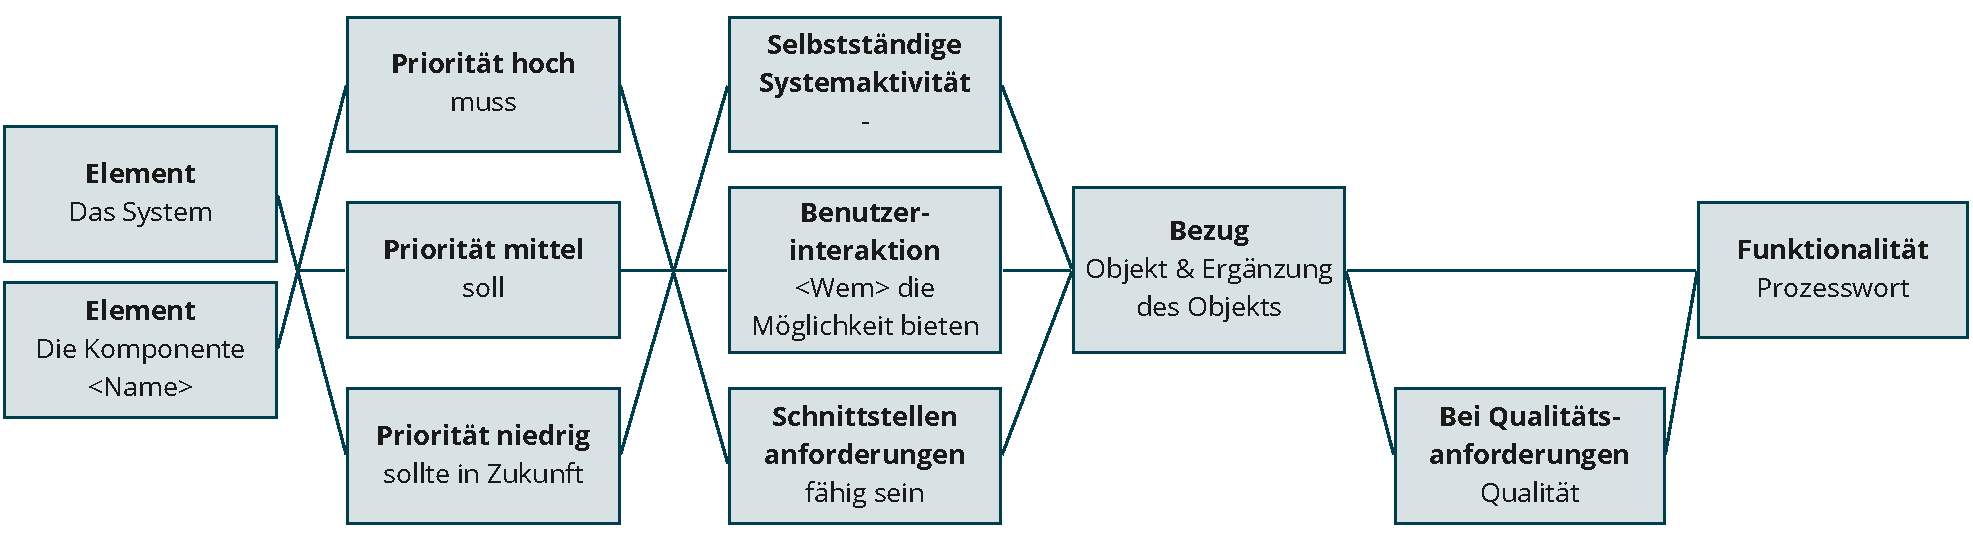
\includegraphics[scale=0.45]{Bilder/anforderungsschablone.pdf}
        \caption[Anforderungsschablone]{Anforderungsschablone \cite{Balzert2009}}
        \label{fig:schablone}
\end{figure}

\newpage
\setanf{F}
\begin{center}
        \renewcommand{\arraystretch}{1.5}
        \begin{longtable}{lp{0.85\textwidth}} \arrayrulecolor{maincolor}\hline
                \anfrow & Das System \textit{muss} Verleihenden und Ausleihenden die Möglichkeit
                bieten, alle Assets jederzeit mittels einer Übersicht einsehen zu können
                \textit{(Ag-Vt-1, \anfref{Z10})}.                                                  \\
                \anfrow & Das System \textit{muss} Verleihenden und Ausleihenden die Möglichkeit
                bieten, die Verfügbarkeit eines Assets einsehen zu können \textit{(Ag-Vt-2,
                \anfref{Z20})}.                                                                    \\
                \anfrow & Das System \textit{muss} Verleihenden und Ausleihenden die Möglichkeit
                bieten, nach Assets zu Filtern und zu Suchen.                                      \\
                \anfrow & Das System \textit{muss}  Verleihenden und Ausleihenden relevante
                Informationen zu den Assets anzeigen (Bild, Name, Beschreibung und Seriennummer)
                \textit{(Ag-Vt-4, Ag-Au-2, \anfref{Z20}, \anfref{Z40})}.
                \\
                \anfrow & Das System \textit{muss}  Ausleihenden relevante Informationen zu
                Ansprechpartner:innen anzeigen \textit{(Ag-Vt-4)}.
                \\
                \anfrow & Das System \textit{muss} Verleihenden und Ausleihenden die Möglichkeit
                bieten, Reservierungen von Assets vornehmen zu können \textit{(Ag-Vt-3)}.
                \\
                \anfrow & Das System \textit{muss} Verleihenden und Ausleihenden die Möglichkeit
                bieten, die verfügbaren Zeitslots der Assets einsehen zu können \textit{(Ag-Vt-2)}.
                \\
                \anfrow & Das System \textit{muss} Ausleihende daran erinnern, die ausgeliehenen
                Assets abzuholen, zurückzubringen oder zu verlängern sind \textit{(Ag-Au-1,
                Ag-Rg-1)}.                                                                         \\
                \anfrow & Das System \textit{soll} Verleihenden und Ausleihenden die Möglichkeit
                bieten, sich mit dem vorhanden IDM (LDAP) Account einzuloggen.
                \\
                \anfrow & Das System \textit{soll} Ausleihenden die Möglichkeit bieten, mittels
                einer Nutzen-Suche individuelle und personalisierte Asset-Vorschläge zu erhalten
                \textit{(Ag-Vt-3, Ag-Au-2)}.
                \\
                \anfrow & Das System \textit{soll} Verleihende automatisch kontaktieren, wenn ein
                Asset reserviert wurde (\textit{Ag-Vt-1}).
                \\
                \anfrow & Das System \textit{soll} Verleihende automatisch erinnern, wenn der
                Zugriff zu einem Asset benötigt wird (\textit{Ag-Au-1}).
                \\
                \anfrow & Das System \textit{soll} Verleihenden und Ausleihenden die Möglichkeit
                bieten, Mängel und Schäden am Asset zu Kennzeichen.
                \\
                \anfrow & Das System \textit{sollte in Zukunft} Verleihenden die Möglichkeit geben
                administrative Aufgaben zu erledigen und an Wartungen zu erinnern
                (\textit{Ag-Rg-2}).                                                                \\
                \anfrow & Das System \textit{sollte in Zukunft} Verleihenden und Ausleihenden die
                Möglichkeit bieten, Assets mithilfe eines QR-Scans in den Reservierung-Checkout zu
                packen.                                                                            \\
                \anfrow & Das System \textit{sollte in Zukunft} Verleihenden und Ausleihenden die
                Möglichkeit bieten, Kommentare und Erfahrungsberichte unter Assets zu schreiben.
                \\
                \anfrow & Das System \textit{sollte in Zukunft} Kommunikation mit Verleihenden
                ermöglichen, sodass keine extra Instanz benötigt wird.
                \\
                \arrayrulecolor{maincolor}\hline
        \end{longtable}
\end{center}

\vspace*{-1.5cm}
\subsection{Qualitätsanforderungen}
\label{section:qualität}
Im letzten Schritt werden die nicht-funktionalen Anforderungen festgelegt, welche die qualitativen
oder quantitativen Eigenschaften eines Systems darstellen \cite{Balzert2009}. Auch hier wird, falls
möglich, die Anforderungsschablone aus \ref{fig:schablone} verwendet.
\setanf{Q}
\begin{center}
        \renewcommand{\arraystretch}{1.5}
        \begin{longtable}{lp{0.85\textwidth}} \arrayrulecolor{maincolor}\hline
                \anfrow & Das System \textit{muss} den Grundsätzen der DIN EN ISO 9241-110:2019-09
                (Ergonomie der Mensch-System-Interaktion - Teil 110: Interaktionsprinzipien) folgen
                (\textit{DIN EN ISO 9241-110}, 2019).
                \\
                \anfrow & Das System \textit{muss} die definierten Nutzungsklassen aus
                \ref{section:benutzer} unterscheiden und die dazugehörigen Zugriffsrechte
                sicherstellen.                                                                       \\
                \anfrow & Das System \textit{muss} zuverlässig und ohne Störung im Dauerbetrieb
                laufen (\nameref{section:zeit}).                                                     \\
                \anfrow & Das System \textit{soll} modular strukturiert sein, damit Inhalte und
                Funktionalitäten effizient eingebunden werden können und das System einfach
                erweiterbar ist.                                                                     \\
                \anfrow & Das System \textit{soll} beim Zugriff über das Internet eine gesicherte
                Übertragung (bspw. \ac{HTTPS}) ermöglichen.
                \\
                \anfrow & Das System \textit{soll} alle Benutzerinteraktionen in unter fünf Sekunden
                ausführen.                                                                           \\
                \arrayrulecolor{maincolor}\hline
        \end{longtable}
\end{center}

%Wie eingangs er-wähnt, definieren die Anforderungen, was das System zu
%leisten hat, während die Funktionalitä-ten definieren, wie das System diese gewährleistet.
\chapter{Konzept}
\label{chapter-konzept}

In diesem Kapitel wird die eigentliche Erkenntnis dieser Arbeit beschrieben. Der Aufbau dieses
Kapitels hängt stark vom Thema der Arbeit ab. Die in dieser Vorlage vorgeschlagenen Kapitel sind
auch nur als Vorschlag und auf keinen Fall als verbindlich zu verstehen.

\section{Funktionalität}




\section{Frameworks} 

\subsection*{Relevante Anforderung an ein Framework}
\subsection*{Wahl des genutzten Frameworks}
Ziel dieser Arbeit ist es, abgeleitet aus den eingangs beschriebenen Anforderungen, ein wirksames
Reservierungstool für Assets zu konzipieren, implementieren und evaluieren. Die Basis für ein
solches Tool schafft die Asset Managementsoftware \textit{SnipeIT} \cite{noauthor_home_nodate},
welche bereits am \ac{imis} eingesetzt wird.

Snipe-IT ist eine kostenlose, quelloffene IT-Asset-Verwaltungs-Plattform,
welche das Nachverfolgen von Software-Lizenzen, Hardware und
Verbrauchsgegenständen ermöglicht. Genannte Assets können über ein Dashboard
hinzugefügt, verwaltet und gelöscht werden. Über Labels können Assets zur
Übersichtlichkeit in verschiedene Kategorien eingeordnet werden, während
Tags ein Asset eindeutig identifizieren (z. B. Seriennummer). Zudem ermöglicht
das „Checkin/Checkout“-System die Nachverfolgung aller Assets, falls diese
z. B.  an Person ausgeliehen werden. Zu jedem Zeitpunkt kann ein Asset
maximal einer Person zugeordnet werden, wodurch das mehrfache gleichzeitige
Ausleihen eines Assets verhindert wird. Darüber hinaus beschreiben Status-Label
den Zustands eines Assets und ob dieses ausgeliehen werden kann. Alle
Funktionalitäten können zudem über eine REST-API programmatisch genutzt werden.


\section{Systemarchitektur}

\section{Interface-Design}

\subsection*{Low-Fidelity-Prototyp}

\subsection*{High-Fidelity-Prototyp}
%Wie eingangs er-wähnt, definieren die Anforderungen, was das System zu
%leisten hat, während die Funktionalitä-ten definieren, wie das System diese gewährleistet.
\chapter{Interface-Design}
\label{chapter-design}
Im Folgenden wurde sich an dem Designprozess Scenario Based Design für die Entwicklung interaktiver
Systeme orientiert. Mithilfe der in \refname{section:iststand} geschilderten Schwierigkeiten konnten
einzelne Szenarien erarbeitet und in Formen einer Vision ausgehend von der aktuellen Situation
formuliert werden \refname{section:funktionale}.

Während des Interface-Designs wurden aus Szenarien Mockups und High-Fidelity-Prototypen entwickelt.
Die Prototypen wurden in Form einer Usability Evaluation direkt getestet: Für die Tests wurden
Usability Spezifikationen aus Szenarien abgeleitet.

Die Szenarien beschreiben Aufgaben die als Vorlage für die Test gestaltung dienen können. Die
Ergebnisse aus den Usability Evaluationen fließen in die weitere Entwicklung mit ein.

Außerdem wurden die Usability Heuristiken nach \citeA{experience_10_nodate} während des gesamten
Prozesses berücksichtigt, um Gebrauchstauglichkeit voraussetzen zu können.

Eine formative Evaluation des Interface-Designs ist wichtig, um früh die Gebrauchstauglichkeit,
die Einfachheit der Bedienung und die Akzeptanz der ästhetischen Gestaltung zu etablieren.



\section{Mockups}

\section{High-Fidelity-Interface-Design}
\subsection{Designsprache}

\subsection{Evaluation der ersten Entwurfs-Iteration}


\begin{table}[h]
    \centering
    \caption{Teilnehmende der Evaluation}
    \begin{tabular}{lll}
            \arrayrulecolor{maincolor}\hline
            \sffamily\color{maincolor}ID & \sffamily\color{maincolor}Alter &
            \sffamily\color{maincolor}Rolle \\
            \arrayrulecolor{maincolor}\hline
            E1                           & 19 - 25 J.                      &
            Medieninformatikerinnen, Hilfswissenschaftlerin                        \\
            E2                           & 19 - 25 J.                      & Roboterinnen \\
            E3                           & 19 - 25 J.                      & ??         \\
            E4                          & 19 - 25 J.                      & ?? \\
            \arrayrulecolor{maincolor}\hline
    \end{tabular}
    \label{table:e}
\end{table}

\todo[inline]{Kriteriensuchen, mehrere Suchen, Wording ändern ->  Eindeutigkeit}

\todo[inline]{Assistent -> Wording: Auswahlhilfe, Suchhilfe, Kriteriensuche, Kiterienhilfe, Auwahl nach Kriterien, Ausleihhilfe
Material statt Assets}

\todo[inline]{Sauber, Clean und nicht überladen}

\todo[inline]{Bei Asset-Suche: Strich bei Kalender: Drawer
Suche und “Kategorien durchstöbern” }



\chapter{Implementierung}
\label{chapter-implementierung}
Das folgende Kapitel beschreibt die Implementierung des Reservierungsinterfaces sowie des Frontends.
Zunächst werden die Implementierung des Reservierungsinterfaces und die damit einhergehenden
technischen Aspekte beschrieben. Dabei wird Aufschluss über die Struktur gegeben und die
Kernfunktionalitäten sowie Herausforderungen in der Realisierung
näher erläutert. Daraufhin wird die Umsetzung des Frontends erläutert. Abschließend wird auf die
Inbetriebnahme des Systems eingegangen.

% Um ein besseres Verständnis für die Interaktion der einzelnen Komponenten zu erlangen, wurde ein
% UML-Sequenzdiagramm erstellt (\ref{fig:uml}). Bei der vierten Komponente handelt es sich um das
% LDAP-System der Universität zu Lübeck. Mithilfe der Integration können Nutzende sich mit ihrem
% bereits bestehenden IDM Account anmelden. Zum einen kann somit sichergestellt werden, dass nur
% befugte Personen Assets einsehen und ausleihen können. Zum anderen erleichtert es den Nutzenden den
% Ausleihprozess, da kein neuer Account erstellt werden muss.

% \begin{figure}[h]
%   \centering
%   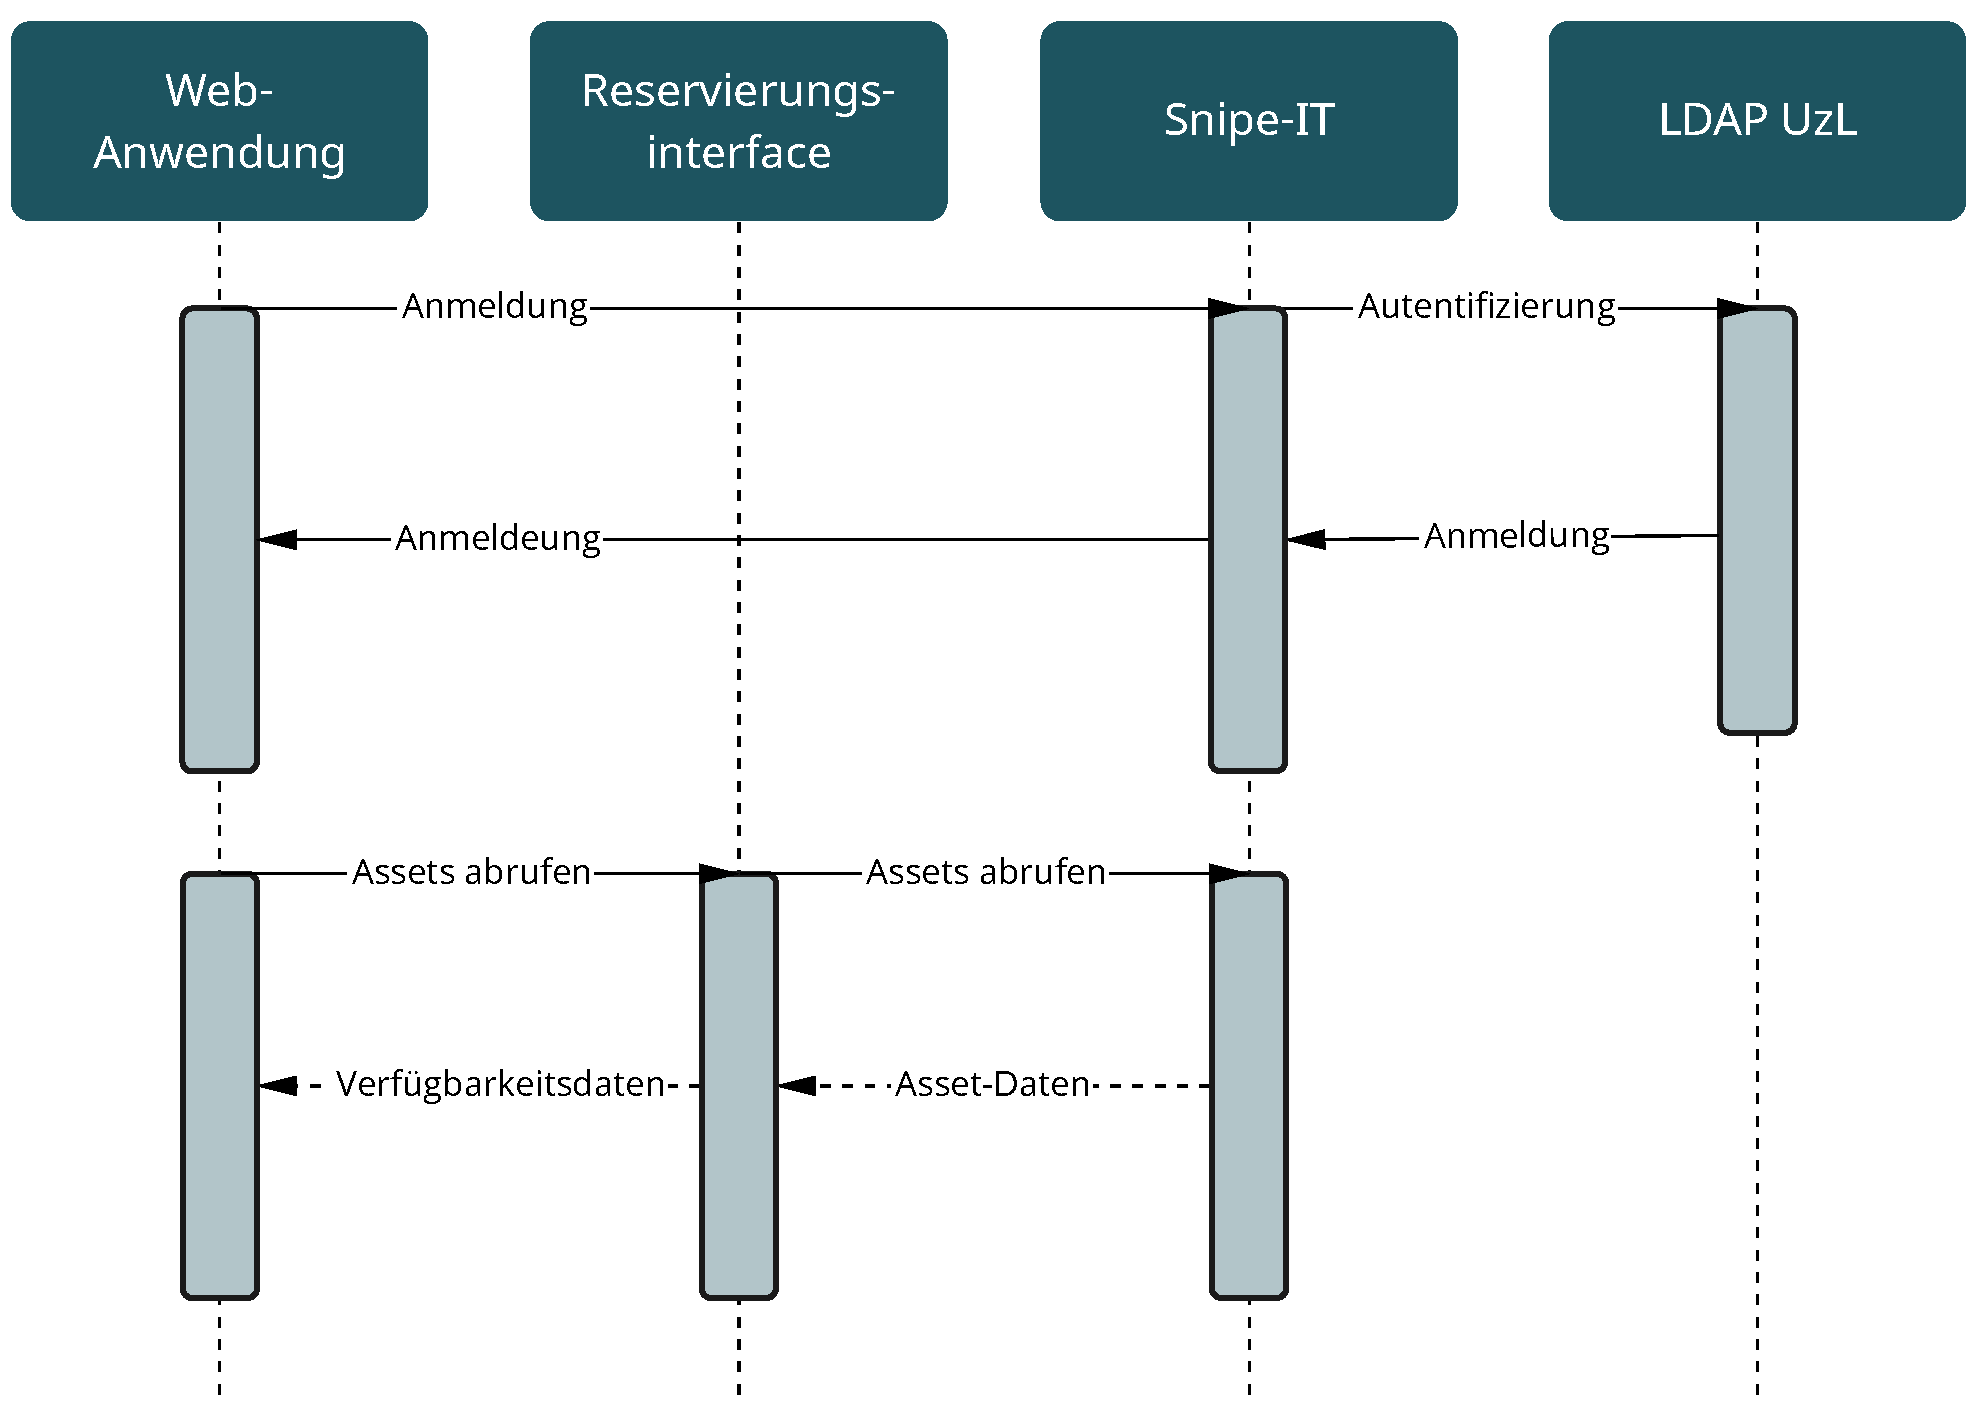
\includegraphics[scale=0.45]{Bilder/uml.pdf}
%   \caption[UML-Sequenzdiagramm]{UML-Sequenzdiagramm}
%   \label{fig:uml}
% \end{figure}


\section{Implementierung des Reservierungsinterfaces}
Dieser Abschnitt erläutert den technischen Aufbau des Rervierungsinterfaces und geht auf relevante
Aspekte in der Realisierung der Kernfunktionalitäten (\ref{section:funktionale}) ein. Des Weiteren
werden unerwartete Herausforderungen thematisiert, welche im Rahmen der Arbeit nicht bewältigt
werden konnten.


\subsection{Aufbau des Reservierungsinterface}
Das Reservierungsinterface teilt sich in drei wesentliche Bestandteile: der
\textit{Fastify-HTTP-Server}, die \textit{SQLite Datenbank} und das \textit{ORM Prisma} (vgl.
\ref{fig:level3}). Diese Komponenten spiegeln sich auch in der Verzeichnisstruktur aus \ref{fig:db}
wider.

\begin{figure}[h]
  \centering
  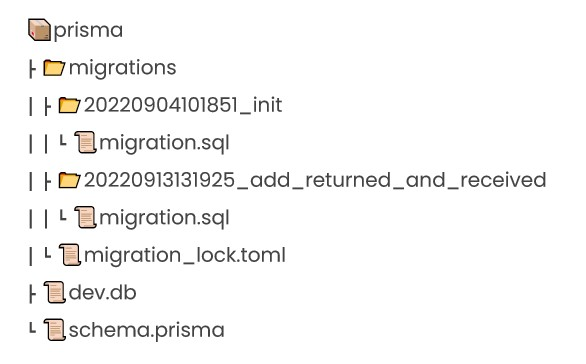
\includegraphics[scale=0.7]{Bilder/Db.jpg}
  \caption[Verzeichnisstruktur des Reservierungsinterfaces]{Verzeichnisstruktur des Reservierungsinterfaces}
  \label{fig:db}
\end{figure}

Der HTTP-Server findet sich in der \textit{server.ts} wieder und stellt dort die API des
Reservierungsinterfaces bereit. Die entwickelte API lässt sich in drei Bereiche teilen:
\textit{Assets}, \textit{Kategorien} und \textit{Reservierungen} (\ref{table:impl-backend-routes}).
Für die drei Inhaltstypen werden die Routen aus \ref{table:impl-backend-routes} bereitgestellt,
welche die von \citeA{fielding_hypertext_2014} beschriebene Semantik für HTTP-Methoden beachten.
Folglich werden bei Verwendung der \textit{GET}-Methode ausschließlich Daten zurückerhalten.
Hingegen muss bei einer Anfrage mit zu übermittelnden Daten die \textit{POST}-Methode verwendet
werden, um einen neuen Eintrag im System zu erschaffen. Beispielsweise wird eine
\textit{GET}-Anfrage an \textit{/assets/:id} abgeschickt, um die Informationen eines Assets zu
erhalten. Um den Status in Snipe-IT auf \textit{herausgegeben} zu aktualisieren, wird eine
\textit{POST}-Anfrage an \textit{/reservation/receive} gesendet, sobald Verleihende eine abgeholte
Reservierung bestätigen.

\begin{table}[h]
  \centering
  \caption{API des Reservierungsinterfaces}
  \begin{tabular}{lll}
    \arrayrulecolor{maincolor}\hline
    \sffamily\color{maincolor}Methode & \sffamily\color{maincolor}Route &
    \sffamily\color{maincolor}Funktion                                                              \\
    \arrayrulecolor{maincolor}\hline
    GET                               & \textit{/assets}                & Erhalte alle Assets       \\
    GET                               & \textit{/assets/:id}            & Erhalte ein Asset mit der
    entsprechende ID                                                                                \\
    GET                               & \textit{/categories}            & Erhalte alle Kategorien   \\
    GET                               & \textit{/reservation}           & Erhalte Reservierungen    \\
    POST                              & \textit{/reservation}           & Erstellen Reservierung    \\
    POST                              & \textit{/reservation/receive}   & Erstellen Reservierung    \\
    POST                              & \textit{/reservation/return}    & Erstellen Reservierung    \\
    POST                              & \textit{/reservation/id}        & Erstellen Erstellen
    Reservierung                                                                                    \\
    DELETE                            & \textit{/reservation/delete}    & Löschen Reservierungen    \\
    PATCH                             & \textit{/reservation/patch}     & Verändern Reservierung    \\
    \arrayrulecolor{maincolor}\hline
  \end{tabular}
  \label{table:impl-backend-routes}
\end{table}

Die mit SQLite bereitgestellte Datenbank speichert die Reservierungen sowie die
Profile. Hierfür wurde das in \ref{fig:orm} dargestellte Datenbankschema
erarbeitet. Zur Umsetzung dieses Schemas wurde das ORM Prisma genutzt, welches
drei zentrale Funktionen bietet.

\begin{figure}[ht]
  \centering
  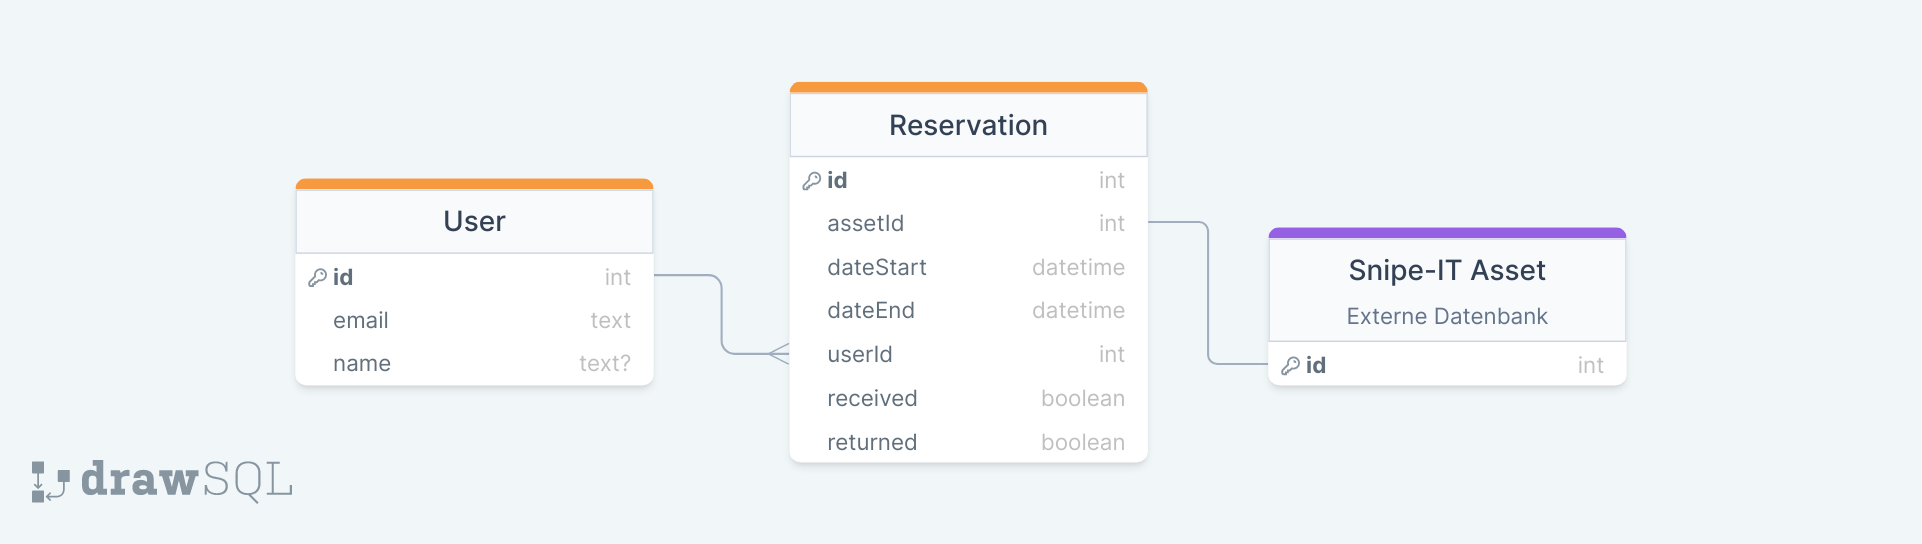
\includegraphics[scale=0.25]{Bilder/drawSQL-export-2022-10-09_15 56.png}
  \caption[Datenstruktur der Reservierungen in Verbindung mit Nutzenden]{Datenstruktur der Reservierungen in Verbindung mit Nutzenden}
  \label{fig:orm}
\end{figure}


\begin{enumerate}
  \item Beschreibung des Schemas durch eigene \ac{dsl} (\ref{fig:prisma})
  \item Automatisierte Migration bei Schemaänderung
  \item JavaScript-Client mit generierten TypeScript-Typen (\ref{fig:mig})
\end{enumerate}

\begin{figure}[h]
  \centering
  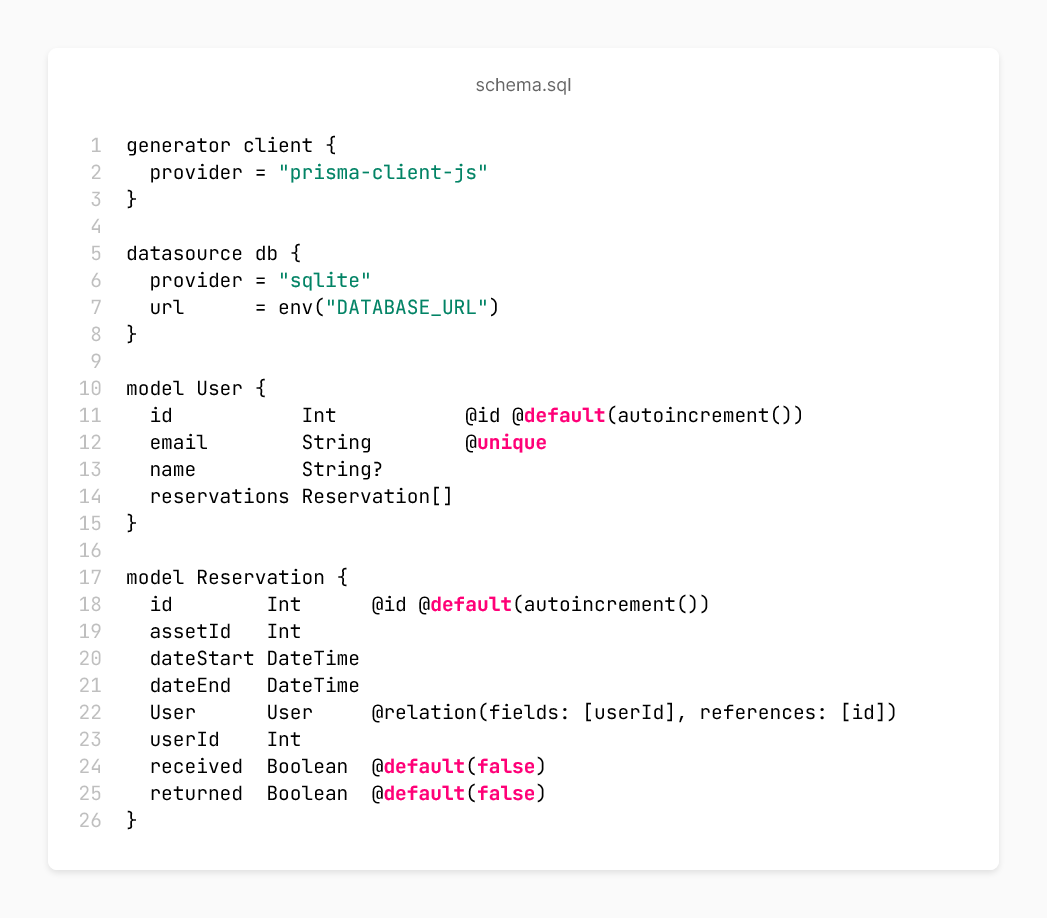
\includegraphics[scale=0.35]{Bilder/screenshot(8).png}
  \caption[Quellcode: schema.prisma]{Quellcode: schema.prisma}
  \label{fig:prisma}
\end{figure}

\begin{figure}[h]
  \centering
  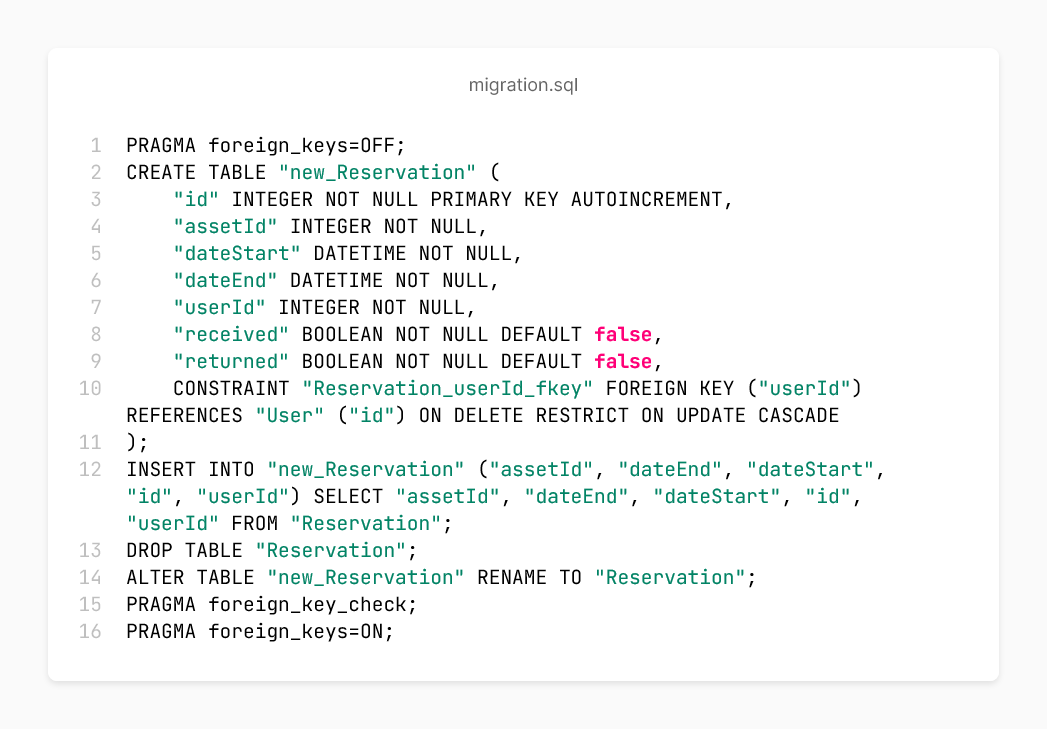
\includegraphics[scale=0.35]{Bilder/screenshot(7).png}
  \caption[Quellcode: migration.sql]{Quellcode: migration.sql}
  \label{fig:mig}
\end{figure}


\subsection{Implementierung der Kernfunktionalität}
Dieser Abschnitt präsentiert die Implementierung der Kernfunktionalität des
Reservierungsinterfaces, welche aus den Anforderungen bestimmt wurde (\ref{section:anforderung}).
Bei der Funktionalität handelt es sich um das Reservieren in die Zukunft, sowie das Speichern
dieser Vorgänge und die damit einhergehende Bestätigung für die Aktualisierung in Snipe-IT.


Sobald ein Asset über die Web-App ausgeliehen wird, werden die relevanten Daten mit einer
\textit{POST}-Anfrage an die \textit{/reservation}-Route des Reservierungsinterfaces gesendet.
Diese relevanten Daten (Assetname, Datum, Uhrzeit, Ort, etc.) werden im Reservierungsinterfaces
gespeichert. Sobald Verleihende die Ausleihe bestätigen, wird der Ausleihstatus mit einer
\textit{POST}-Anfrage an \textit{/reservation/receive} intern und in Snipe-IT von
\textit{ausleihbar} zu \textit{herausgegeben} aktualisiert. Zur Kommunikation zwischen dem
Reservierungsinterface und Snipe-IT wird das Paket \textit{node-fetch} genutzt, welches die
Fetch-API des Browsers in \textit{Node.js} bereitstellt. Für das Aktualisieren des Status eines
Assets mit der \textit{assetId} wird beispielsweise eine \textit{POST}-Anfrage an
\textit{<SnipeIt\_URL>/api/v1/hardware/<assetId>/checkout} versendet, welche die ID des
\textit{herausgegeben}-Status und die ID des ausleihenden Nutzenden beinhaltet (\ref{fig:server}).
Analog geschieht dies für das Zurückgeben eines Assets mit einer \textit{POST}-Anfrage an
\textit{/reservation/return}.

\begin{figure}[h]
  \centering
  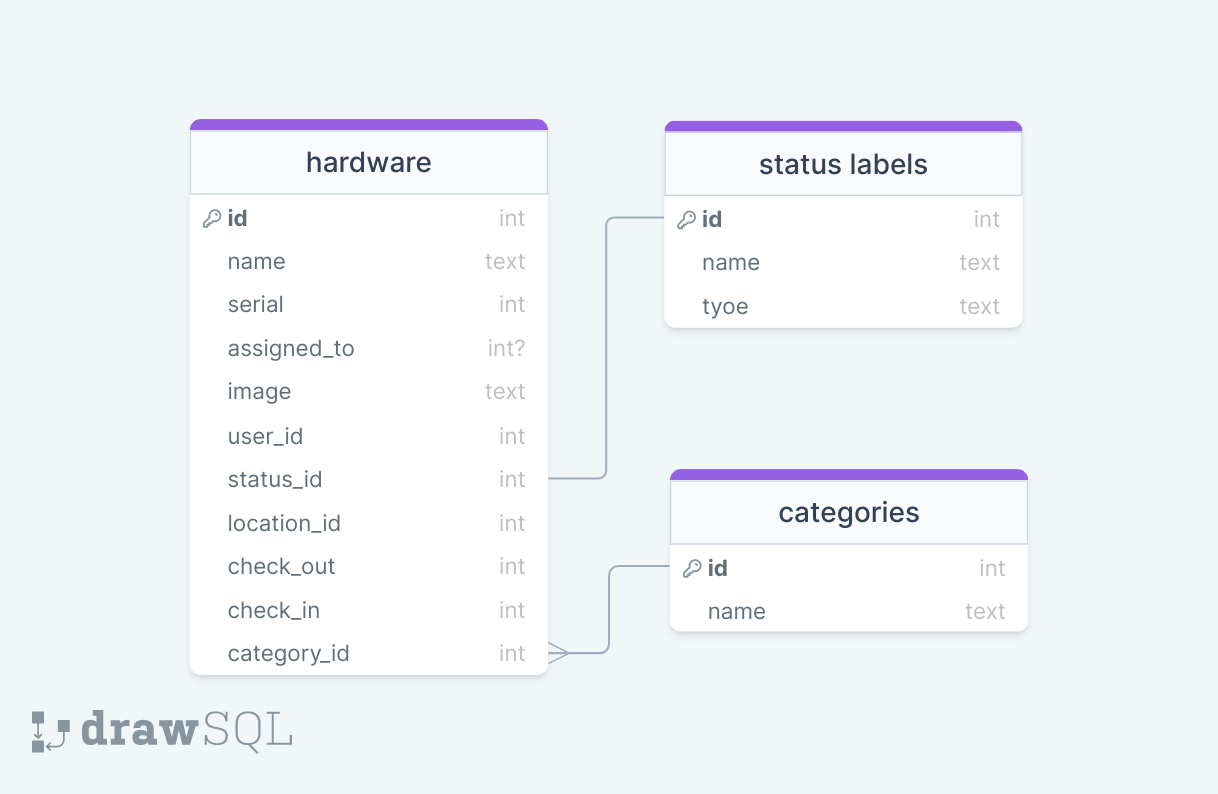
\includegraphics[scale=0.3]{Bilder/apisnipeit.png}
  \caption[UML Snipe-IT API]{UML Snipe-IT API}
  \label{fig:server}
\end{figure}

Um auf die Assets zugreifen zu können, wurde mit der Snipe-IT JSON REST API gearbeitet. Die Snipe-IT
API umfasst viele Routen\footnote{\url{https://snipe-it.readme.io/reference/api-overview}} für die
Abfrage und Manipulation der internen Datenbank, wovon \textit{/hardware, /categories} und
\textit{/statuslabels} relevant für die Umsetzung dieser Arbeit waren. \ref{fig:snipe} zeigt den
Aufbau und die Beziehungen der genutzten Snipe-IT API Ressourcen, wobei die Ressource
\textit{hardware} den Assets in der Snipe-IT Datenbank entspricht.

\begin{figure}[h]
  \centering
  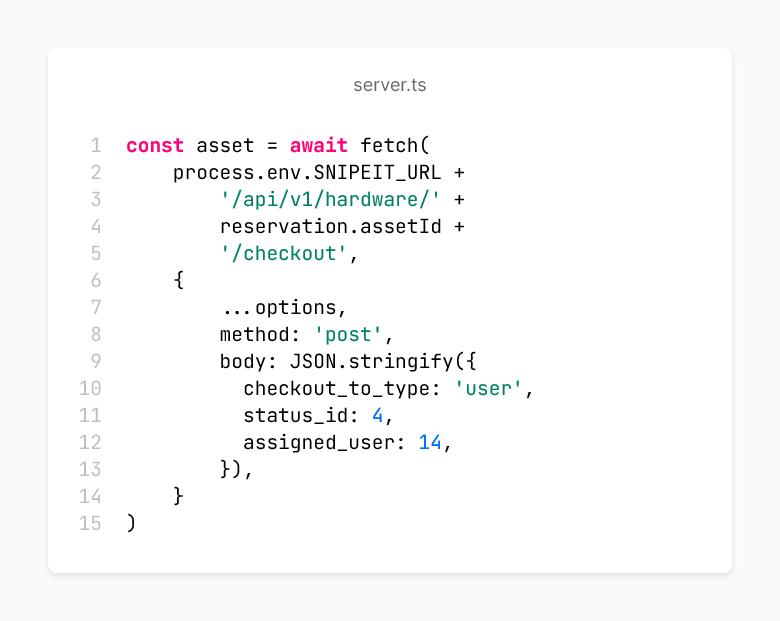
\includegraphics[scale=0.4]{Bilder/screenshot(5).png}
  \caption[Quellcode: server.ts]{Quellcode: server.ts}
  \label{fig:snipe}
\end{figure}

Um mit der API arbeiten zu können, muss ein \textit{persönliches
  Zugriffstoken}\footnote{\url{https://snipe-it.readme.io/reference/generating-API-tokens}} für die
Nutzung generiert werden. Das persönliche Zugriffstoken muss mit jeder Anfrage an die API, in Form
eines \lstinline{Bearer <Token>} HTTP-Headers, mitgeschickt werden. Da persönliche Zugriffstoken
verwendet werden, spiegeln die Berechtigungen des API-Tokens die Berechtigungen des Nutzenden
wider.

\subsection{Herausforderungen in der Einbindung von LDAP}
Snipe-IT bietet bereits eine integrierte Lösung zur Synchronisation und Login mit
LDAP\footnote{\url{https://snipe-it.readme.io/docs/ldap-sync-login}}. Da die \textit{persönlichen
  Zugriffstoken} jedoch die einzige Authentifizierungsmöglichkeit der API sind und lediglich manuell
im Dashboard generiert werden können, kann das LDAP-System der Universität zu Lübeck nicht ohne
Umstände eingebunden und entsprechend genutzt werden.

Ein möglicher Lösungsansatz wäre das programmatische Nutzen eines Browsers aufseiten des
Reservierungsinterfaces, welcher die Angaben von Nutzenden in der Wep-App verwendet, um mit diesen
den LDAP-Login in Snipe-IT durchzuführen. Sollte der Snipe-IT Login erfolgreich sein, könnten
Nutzende für den Rest der Sitzung als authentifiziert gelten. Im Reservierungsinterface selbst
würde ein speziell für das Reservierungsinterface generierte Token für die Kommunikation mit
Snipe-IT genutzt werden.

\section{Implementierung des Frontends}
Das kommende Kapitel beschreibt die Client-seitige Realisierung der Arbeit. Zunächst wird der Aufbau
betrachtet, daraufhin wird auf das Extrahieren der Unterkategorien eingegangen (\ref{fig:vue}).


Für den Aufbau des Projektes wurde aus den in \ref{chapter-konzept} festgestellten Anforderungen
\textit{vue.js} verwendet. Bei der Implementierung wurde sich an den best practices der
Vue.js-Dokumentation orientiert \todo{(Vue.js, 2021a)}. Für sich wiederholende Elemente wurden
eigene Views erstellt. Dadurch ergibt sich eine hierarchisch geschachtelte Client-Anwendung der
Vue-Komponenten. \ref{fig:vue} stellt die Komponenten-Struktur vereinfacht dar. Um
konkretere Vorschläge in der Entwicklungsumgebung zu ermöglichen und vorzeitige Fehler zu
minimieren, wurde ergänzt zu \textit{JavaScript} \textit{TypeScript} verwendet.

\subsection{Aufbau der Routen und Komponentenstruktur}
Für die Realsisierung der Routen wurde der File-Based-Routing Ansatz verwendet, welcher die Routen
aufgrund der Verzeichnisstruktur generiert. Hierfür wurde das Vite-Plugin
\textit{vite-plugin-pages}\footnote{\url{https://github.com/hannoeru/vite-plugin-pages}} genutzt.
Vue-Komponenten, welche sich im \textit{/pages}-Verzeichnis des Projekts befinden, werden in eine,
dem Dateinamen gleichende, Route umgewandelt. Ordner können hierbei verwendet werden, um Unterrouten
zu erstellen, während die Verwendung von eckigen Klammern zur Kennzeichnung von Parametern genutzt
wird\todo{Der vorherige Statz=DOOF}. Beispielsweise wird eine \textit{[id].vue}-Datei, welche sich
in dem Ordner \textit{categories} befindet, in die \textit{/categories/<id>}-Route umgewandelt,
welche die angegebene ID in der Komponente als Parameter nutzen kann (\ref{fig:vue}).

\begin{figure}[h]
  \centering
  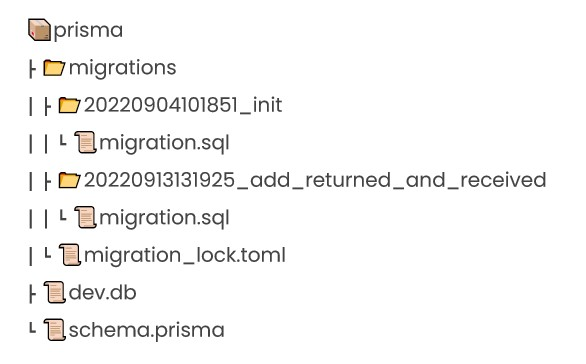
\includegraphics[scale=0.7]{Bilder/Db.jpg}
  \caption[Verzeichnisstruktur des Clients]{Verzeichnisstruktur des Clients}
  \label{fig:vue}
\end{figure}

\subsection{Extrahieren von Unterkategorien}
Die im Rahmen dieser Arbeit verwendete Beispieldatenbank beinhaltete eine Vielzahl an Kategorien und
Unterkategorien welche nach folgendem Format benannt wurden: \enquote{Kategorie - Unterkategorie}.
Das verwendete Format ergibt sich aus der fehlenden Funktionalität Snipe-Its, einem Asset mehrere
Kategorien zuweisen zu können. Da das Anzeigen der Kategorien in diesem Format unübersichtlich ist,
sollten zunächst nur die Oberkategorien und anschließend die Unterkategorien angezeigt werden.
\ref{fig:categoriecode} stellt eine vereinfachte Form des verwendeten Quellcodes dar.

\begin{figure}[h]
  \centering
  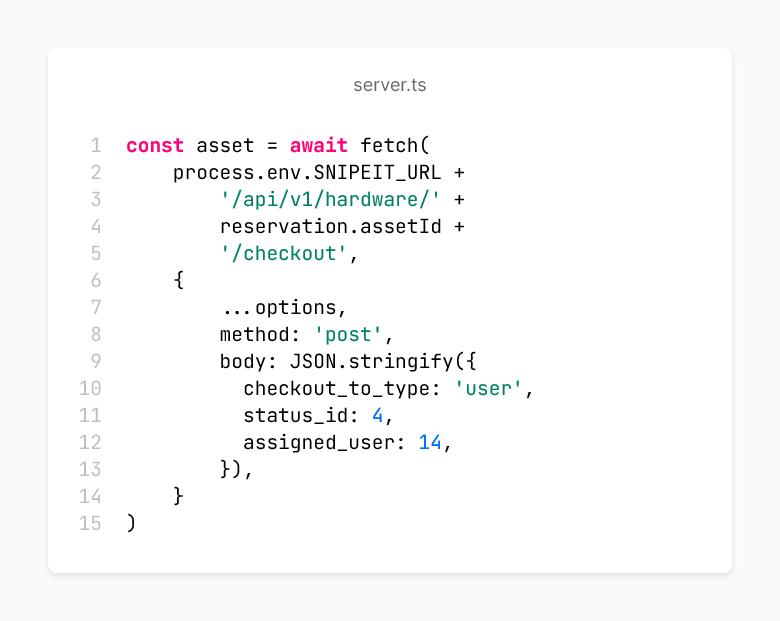
\includegraphics[scale=0.4]{Bilder/screenshot(5).png}
  \caption[Quellcode: server.ts]{Quellcode: server.ts}
  \label{fig:categoriecode}
\end{figure}

Zur Extrahierung werden die erhaltenen Kategorien, anhand eines Trennsymbols (\enquote{-}), in Ober- und
Unterkategoriepaare getrennt. Anschließend werden alle Paare mit der gleichen Oberkategorie zu einem
Eintrag zusammengefasst, welcher alle zugehöhrigen Unterkategorien beinhaltet. Hierbei wird für jede
Unterkategorie die hinterlegte Kategorie-ID gespeichert. Somit ergibt sich eine Baumstruktur, welche
in der Anwendung schrittweise durchlaufen werden kann.


\section{Nutzung des Systems}
Der folgende Abschnitt führt die nötigen Schritte auf, um das System in Betrieb nehmen zu können.
Zuerst wird die Installation erklärt, gefolgt von der Konfiguration und Ausführung des Systems.

\subsection{Installation}
Für die Nutzung des Systems wird eine Installation von \textit{Node.js} vorausgesetzt. Zunächst
müssen alle eingebundenen Pakete des \textit{npm} Paketverzeichnis mit \lstinline{npm install}
installiert werden. Dies muss für Server (\lstinline{\server}) und Client (\lstinline{\client})
jeweils im entsprechenden Verzeichnis ausgeführt werden. Zusätzlich sollte die Datenbank im
Server-Verzeichnis mithilfe des Befehls \lstinline{npx prisma install }\todo{Befehl raussuchen}
erstellt und vorbereitet werden. Abschließend sollte \lstinline{npx prisma generate} ausgeführt
werden, um die benötigten Datein des Prisma-Clients zu generieren.

\subsection{Konfiguration}
Zur Festlegung von umgebungsabhängigen Variablen werden für Server und Client je eine
\textit{.env}-Datei verwendet. Diese müssen vor der Inbetriebnahme angelegt werden und sind nach dem
Schema in BILD aufgebaut. Der Server benötigt die URL der zu verwendenden Snipe-IT Instanz, den
API-Key zur Authentifizierung (\ref{section:api}) und den Pfad der SQLite Datenbankdatei.
Aufseiten des Clients wird lediglich die URL des Reservierungsinterfaces benötigt.

\begin{figure}[h]
  \centering
  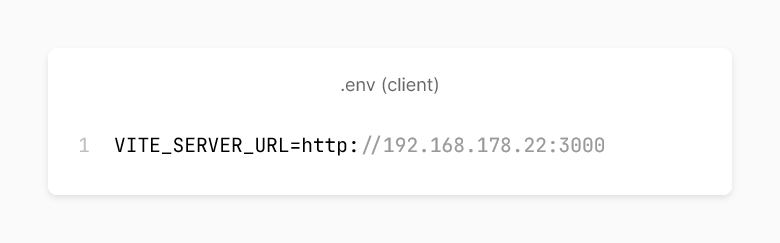
\includegraphics[scale=0.25]{Bilder/client.png}
  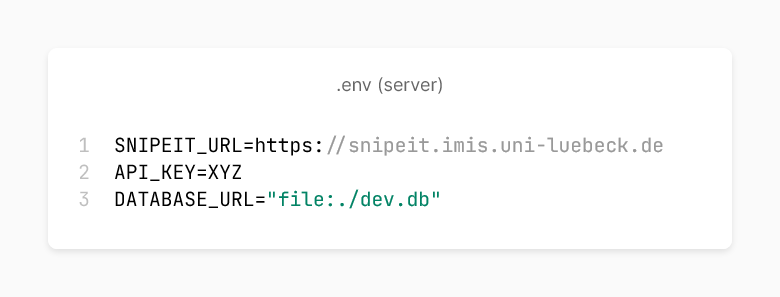
\includegraphics[scale=0.25]{Bilder/sever.png}
  \caption[Inhalte der .env Datei im Frontend (links) und Backend (rechts)]{Inhalte der .env Datei im Frontend (l) und Backend (r)}
  \label{fig:env}
\end{figure}


\subsection{Einrichtung des Snipe-IT API-Zugangs}
\label{section:api}
Um die gewünschte(n) Datenbank(en) aus Snipe-IT nutzen zu können, wird ein Account in Snipe-IT
benötigt, welcher von Administrierenden angelegt werden muss. Daraufhin muss über die
Profileinstellung \textit{Manage API Keys} ein API-Key generiert werden. Der generierte API kann nun
in der Konfiguration genutzt werden. Außerdem sollte beachtet werden, dass der API Key nur einmalig
nach der Generierung einsehbar ist.

\subsection{Ausführung des Reservierungsinterfaces}
\begin{itemize}
  \item Ausführung per \lstinline{npm run serve}
\end{itemize}
\todo{ausformulieren}

\subsection{Ausführung der Web-App}
Das Ausführen und "bauen" der Web-App geschieht über den Befehl \lstinline{npm run build-only}.
Nachdem der Prozess erfolgreich abgeschlossen ist, sollte ein neues \textit{dist}-Verzeichnis
generiert worden sein. Das \textit{dist}-Verzeichnis kann zum statischen Hosting genutzt werden.


\section{Fazit der Implementierung}

Die in der Implementierung realisierten Funktionalitäten umfassen das \textit{muss} der in der
\nameref{section:anforderung} erarbeiteten Funktionen.
\todo{ quasi alle Unterüberschriften in einem Satz zusammenfassen, sodass jemand, der das Kapitel nicht gelesen hat, grob ne Idee davon hat, was hier abging}

\chapter{Dialogbeispiel}
\label{chapter-dialogbeispiel}

Der folgende Abschnitt präsentiert das in der vorliegenden Arbeit realisierte System anhand eines
beispielhaften Nutzungsszenarios. Das Szenario Start mit Mila, einer Erstsemester Studentin im
Studiengang Medieninformatik. Mila belegt im ersten Semester das Modul \textit{\ac{emi}}. Das
Einführungsmodul umfasst eine Gruppenarbeit, in der zum Thema \textit{VR/AR} eine Idee entwickelt
werden soll. Am Ende des Semesters soll das Projekt bei den \textit{Media Moments} in der
\textit{\ac{emi} Award App}\footnote{RAIMUNDS BA HEHE} ausgestellt werden. Milas Projektgruppe hat
sich entschieden eine AR-Anwendung für Erze und Metalle zu gestalten, bei der die Erze und Metalle
mithilfe einer App eingescannt werden können und die entsprechenden Eigenschaften angezeigt werden.
Um das Projekt in der \textit{\ac{emi} Award App} präsentieren zu können, will die Gruppe ein
Werbevideo für die App aufnehmen.

In einem Videoworkshop von Georg Fink, fiktiver \ac{wimi} am \ac{imis}, erfahren Mila und ihre
Gruppenmitglieder, dass unter anderem Videoequipment über die Ausleih-App \textit{Snipe-IT Companion} an
Studierenden verliehen wird.

Mila ruft die Ausleih-App unter der URL \textit{https://snipe-it-companion.de/} auf und meldet
sich mit ihren \todo{LDAP-} Daten an. Daraufhin wird sie zu einem bisher leeren \textit{Dashboard}
weitergeleitet und aufgefordert nach benötigtem Material zu suchen. Da Mila sich nicht sicher ist,
welche Kamera sie benötigt, schaut sich Mila unter dem Menü, in den Kategorien um und findet
schnell die Kategorie \enquote{Kameras}. Nachdem sie auf die Seite der Unterkategorien
weitergeleitet wurde, entscheidet sich Mila dafür eine \textit{GoPro} auszuleihen, weil sie so auch
Erze und Metalle unter Wasser aufnehmen können, dazu klickt Mila auf \enquote{Hinzufügen}.

\begin{figure}[h]
    \centering
    \includegraphics[scale=0.3]{Bilder/Prototyp/Übersicht.png}\hspace{2em}
    \includegraphics[scale=0.3]{Bilder/Prototyp/Übersicht1.png}
    \label{fig:p4}
    \caption[Mockup: Kategorien, Assets, Assetdetails]{Kategorien (l), Assetdetails (r)}
\end{figure}

Nun wird sie dazu aufgefordert einen Ausleihzeitraum anzugeben. Milas Gruppe hat entschieden, dass
sie von kommendem Montag bis Mittwoch das Material benötigten. Da Mila von 8:00 Uhr bis 10:00 Uhr
eine Vorlesung hat, gibt sie 10:30 Uhr als Abholzeit sowie als Rückgabezeit an. Um die Reservierung
abschließen zu können, klickt Mila auf \enquote{Reservieren}. Mila überprüft in der Zusammenfassung,
ob ihre Angaben stimmen und stellt fest, dass die Rückgabezeit am Mittwoch doch nicht mehr in ihren
Kalender passt, daher ändert sie die Uhrzeit auf 12:30 Uhr. Abschließend bestätigt Mila ihre
Reservierung.

Da sich die Gruppe nicht sicher ist, welches Mikrofon für die Aufnahme eines Voiceover sinnvoll ist,
suchen sie zunächst in der Ausleih-App nach Mikrofon und sehen das Georg Fink für diese zuständig ist.
Daraufhin schreibt Mila Herrn Fink eine E-Mail, welches Mikrofon Georg für ein Voiceover empfehlen würde.
Georg gibt in seiner Antwort zwei Vorschläge. Nachdem Mila Herrn Finks Antwort erhalten hat, gibt sie in
der Suche den Ausleihzeitraum ein und sucht nach Herrn Finks Vorschlägen. Direkt stellt Mila fest, dass nur
eines der Mikrofone in dem Ausleihzeitraum ausleihbar ist und reserviert dieses.

Georg ist als fiktiver \ac{wimi} am \ac{imis} für zwei Labore zuständig, in denen Material
ausgeliehen werden kann. Zum Feierabend überprüft er sein Verwaltungsdashboard auf dem Desktop in
der Ausleih-App. Er sieht, das eine neue Reservierung für Montag um 10:30 Uhr von Mila eingegangen
ist.

\begin{figure}[h]
    \centering
    \includegraphics[scale=0.3]{Bilder/Prototyp/Übersicht.png}
    \label{fig:p4}
    \caption[Mockup: Kategorien, Assets, Assetdetails]{Kategorien (l), Assetdetails (r)}
\end{figure}

Da sich Mila am Sonntag nicht sicher ist, wo der Abholort der Materialien ist, schaut sie
erneut in der Ausleih-App nach und findet diesen auf der Dashboardansicht.

\begin{figure}[h]
    \centering
    \includegraphics[scale=0.3]{Bilder/Prototyp/Übersicht.png}\hspace{2em}
    \includegraphics[scale=0.3]{Bilder/Prototyp/Übersicht1.png}
    \label{fig:p4}
    \caption[Mockup: Kategorien, Assets, Assetdetails]{Kategorien (l), Assetdetails (r)}
\end{figure}

Nach der Vorlesung am Montag macht sich Mila auf den Weg in das Gebäude 64 zum Abholort: Techniklabor.
Georg wartet dort bereits auf Mila und erklärt ihr, was sie bei der \textit{GoPro} beachten sollte.
Nachdem Mila gegangen ist, trägt Georg auf seinem Smartphone ein, dass die Materialien abgeholt wurden.
Sobald Georg die Abholung bestätigt hat, wird der Status in der internen Datenbank Snipe-IT
geändert.

\begin{figure}[h]
    \centering
    \includegraphics[scale=0.3]{Bilder/Prototyp/Übersicht.png}\hspace{2em}
    \includegraphics[scale=0.3]{Bilder/Prototyp/Übersicht1.png}
    \label{fig:p4}
    \caption[Mockup: Kategorien, Assets, Assetdetails]{Kategorien (l), Assetdetails (r)}
\end{figure}

Laura Eggers ist ebenfalls fiktive \ac{wimi} am \ac{imis} und möchte für eine Studie ein Mikrofon
ausleihen, da sie Zugriff auf Snipe-IT hat, schaut sie zunächst dort nach dem gewünschten Material
und stellt fest, dass dieses \textit{herausgegeben} ist. Daraufhin ruft sie die URL
\textit{https://snipe-it-companion.de/} auf und reserviert das Mikrofon im gewünschten Zeitraum.
Am Abholtag entnimmt sie das Asset und bestätigt die Abholung auf ihrem Smartphone.

\begin{figure}[h]
    \centering
    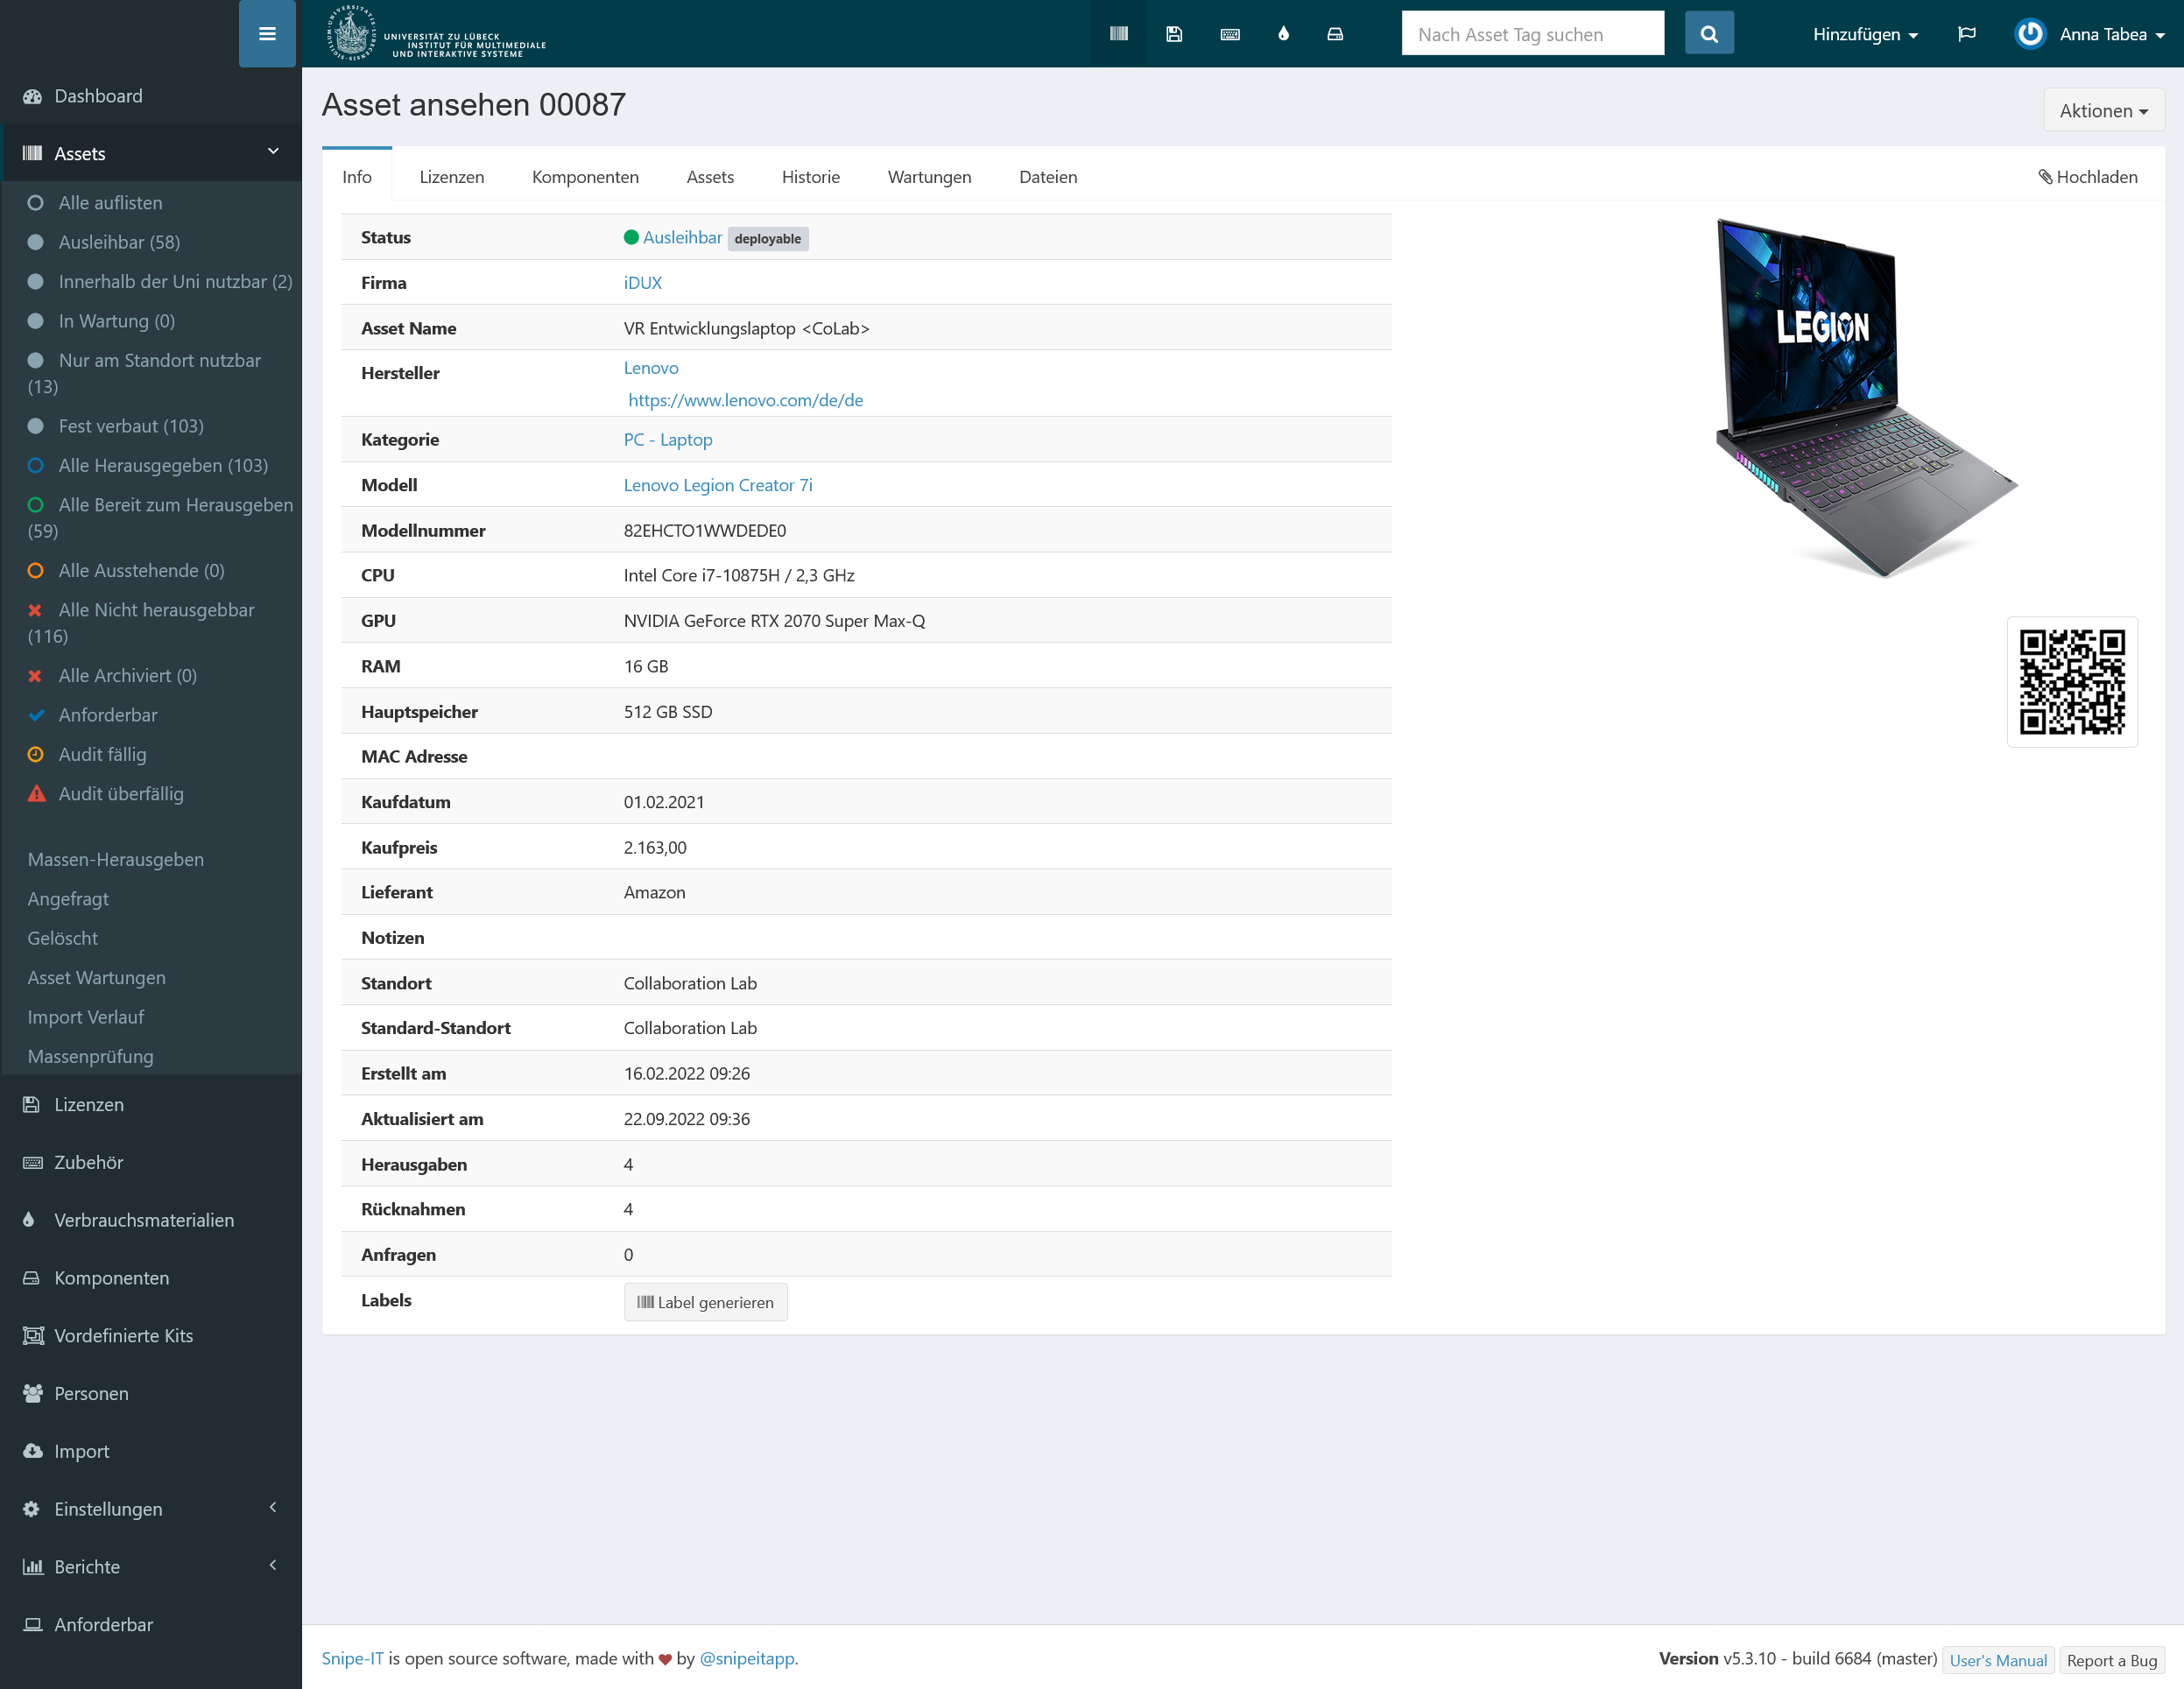
\includegraphics[scale=0.16]{Bilder/Screenshot 2022-10-14 at 11-26-25 Asset ansehen 00087 Ausleihmanagement.png}
    \label{fig:p4}
    \caption[Assetansicht in Snipe-IT]{Assetansicht in Snipe-IT}
\end{figure}

Milas Gruppe stellt am Dienstag fest, dass ihnen der Ausleihzeitraum nicht ausreicht und möchte
diesen daher um einen Tag verlängern. Dafür öffnet sie die Ausleih-App und sieht auf dem Dashboard
unter \textit{Laufende} ihre Reservierungen. Daraufhin ändert sie die Daten der beiden Materialien
auf Donnerstag um 9:00 Uhr. Am Donnerstag um 9:00 Uhr wartet Mila bereits auf Georg, welcher die
Materialien entgegennimmt und in seinem Büro die Rückgabe bestätigt.

\begin{figure}[h]
    \centering
    \includegraphics[scale=0.3]{Bilder/Prototyp/Übersicht.png}\hspace{2em}
    \includegraphics[scale=0.3]{Bilder/Prototyp/Übersicht1.png}
    \label{fig:p4}
    \caption[Mockup: Kategorien, Assets, Assetdetails]{Kategorien (l), Assetdetails (r)}
\end{figure}

Im vierten Semester möchte Mila das Mikrofon für das Modul: \textit{\ac{ide}} ausleihen, um wieder
ein Voiceover aufnehmen zu können. Sie findet das Mikrofon unter \textit{zurückgegeben} und
leiht das Material erneut aus.

\begin{figure}[h]
    \centering
    \includegraphics[scale=0.3]{Bilder/Prototyp/Übersicht.png}\hspace{2em}
    \includegraphics[scale=0.3]{Bilder/Prototyp/Übersicht1.png}
    \label{fig:p4}
    \caption[Mockup: Kategorien, Assets, Assetdetails]{Kategorien (l), Assetdetails (r)}
\end{figure}
%!TEX root = thesis.tex

\chapter{Evaluation}
\label{chapter-evaluation}

In der Evaluierung wird das Ergebnis dieser Arbeit bewertet. Eine praktische Evaluation eines neuen Algorithmus kann zum Beispiel durch eine Implementierung geschehen. Je nach Thema der Arbeit kann sich natürlich auch die gesamte Arbeit eher im praktischen Bereich mit einer Implementierung beschäftigen. In diesem Fall gilt es am Ende der Arbeit insbesondere die Implementierung selber zu evaluieren. Wesentliche Fragen dabei können sein:
\begin{compactitem}[--]
  \item Was funktioniert jetzt besser als vor meiner Arbeit?
  \item Wie kann das praktisch eingesetzt werden?
  \item Was sagen potenzielle Anwender zu meiner Lösung?
\end{compactitem}

\section{Vorgehen und Methodik}
- Wording mit Abfragen

\section{Verleihende}

\section{Ausleihende}

Wenn Implementierungen umfangreich beschrieben werden, ist darauf zu achten, den richtigen Mittelweg zwischen einer zu detaillierten und zu oberflächlichen Beschreibung zu finden. Eine Beschreibung aller Details der Implementierung ist in der Regel zu detailliert, da die primäre Zielgruppe einer Abschlussarbeit sich nicht im Detail in den geschriebenen Quelltext einarbeiten will. Die Beschreibung sollte aber durchaus alle wesentlichen Konzepte der Implementierung enthalten. Gerade bei einer Abschlussarbeit am Institut für Softwaretechnik und Programmiersprachen lohnt es sich, auf die eingesetzten Techniken und Programmiersprachen einzugehen. Ich würde in einer solchen Beschreibung auch einige unterstützende Diagramme erwarten.


\section{Diskussion}
%!TEX root = thesis.tex

\chapter{Zusammenfassung und Ausblick}
\label{chapter-fazit}

Abschließend werden die wichtigsten Ergebnisse und Antworten auf die
Forschungsfragen (\ref{sec:Forschungsfragen}) der vorliegenden Arbeit
zusammengefasst. Im Anschluss werden offene Punkte der Konzeption, welche nicht
wie geplant umgesetzt werden konnten, erläutert. Zum Abschluss wird auf die
möglichen Weiterentwicklungen des entwickelten Systems eingegangen.


\section{Zusammenfassung}
Für den Ausleih- und Reservierungsprozess ist die Unterstützung durch ein
Reservierungstool eine zielführende Möglichkeit, um die Planung in die Zukunft
zu erleichtern und zu ermöglichen. Hierbei ist insbesondere eine strukturierte und
übersichtliche Ansicht der auszuleihenden Assets von hoher Bedeutung.

Um ein solches Konzept entwickeln zu können, wurden zunächst aus vorangestellten
Untersuchungen die objektiven Anforderungen an den Snipe-IT Companion erarbeitet
und formalisiert (\ref{section:anforderung}). Die wichtigste Informationsquelle
stellten hierbei die Stakeholder-Interviews mit Mitarbeitenden des \ac{imis} und
Studierenden der Medieninformatik dar. Zusätzlich wurde eine Recherche zu
vergleichbaren Systemen vorgenommen, welche Aufschluss über mögliche
Fehlerquellen geben sollte. Hierbei wurde sich nach einer weiteren Recherche auf
zwei in den Interviews genannten Apps beschränkt, da die vorherige Recherche
wenig Aufschluss für den spezifischen Einsatzfall gab. Aus den Quellen konnten
zwei Nutzendengruppen (Verleihende und Ausleihende) erarbeitet werden
(\ref{section:Nutzenden}). Für Forschungsfrage F1 wurden die Probleme und
Herausforderungen des aktuellen Vorgehens und de unterschiedlichen
Ausleihprozesse, in einer Problemanalyse erarbeitet und beantwortet
(\ref{section:iststand}). Anschließend wurden die Aufgaben, welche Verleihende
und Ausleihende im Reservierungsprozess erledigen müssen, zur Vorbereitung für
Forschungsfrage F2 diskutiert (\ref{section:aufgaben}).

In der Spezifikationsphase wurden die Anforderungen an das System weiter
eingegrenzt (\ref{chapter-konzept}). Dazu wurden gemäß der Forschungsfrage F2 zunächst
Funktionalitäten definiert. Die Funktionalitäten wurden entsprechend
den Anforderungen entwickelt und in einer priorisierten Feature-Liste
festgehalten. Anschließend wurde die Systemarchitektur, aufgeteilt in Frontend,
Reservierungsinterface (Backend) und dem bestehenden Snipe-IT Server, mithilfe
des C4-Models dargestellt (\ref{section:architektur}). Aufbauend darauf wurden
passende Frameworks zur Entwicklung ausgewählt.

Aufbauend auf dem Konzept wurde das Interface-Design erarbeitet
(\ref{chapter-design}). Durch das regelmäßige Einarbeiten von Interviews konnte
ein iteratives Vorgehen ermöglicht werden. Daraus resultierten zentrale
Designentscheidungen wie die Wahl der Begrifflichkeiten oder die Navigation, welche in
Folgearbeiten berücksichtigt werden sollten.

Mithilfe der vorangestellten Phasen wurde das Reservierungstool entsprechend
umgesetzt (\ref{chapter-implementierung}). Hierbei wurden die in der
Konzeptionsphase festgelegten Frameworks genutzt. \ref{chapter-dialogbeispiel}
präsentiert das realisierte System anhand von Dialogbeispielen.

In der abschließenden Phase wurde das realisierte System mithilfe von Interviews
und Umfragen evaluiert (\ref{chapter-evaluation}). Die Ergebnisse der Phase
dienten zur Beantwortung von Forschungsfrage F3 und gaben Aufschluss über die
Wirksamkeit des entwickelten Systems. Generell wurde die Oberfläche als
übersichtlich beschrieben und der Wunsch, die Anwendung im Universitätsalltag
für Projekte nutzen zu können, geäußert. Die eingangs formulierte Forschungsfrage
F3 konnte lediglich bedingt beantwortet werden, da das positive Ergebnis der
durchgeführten Studie nicht verglichen werden konnte. Eine weitere ausführliche
Studie mit einem Vergleichsystem wird somit empfohlen. Trotz des fehlenden
Vergleichs konnte die Arbeit ein qualitativ hochwertiges System hervorbringen,
welches sich als übersichtlich und unterstützend herausstellt. Für
Forschungsfrage 2 konnten weitere Anforderungen an das System herausgearbeitet
werden.

\section{Offene Punkte}
\label{sec:punkte}
Die in den Anforderungen festgelegten Funktionalitäten mit hoher Prioriät
konnten umgesetzt werden. Die mittel priorisierten Funktionalitäten stellten
sich als Herausforderung raus. Insbesondere \anfref{F90}, die Einbindung des
\ac{ldap}-Systems, führte zu Schwierigkeiten und wurde dementsprechend nicht
umgesetzt. Zentrale Gründe hierfür waren der \textit{persönliche
    Zugriffstoken}, welcher die einzige Authentifizierungsmöglichkeit der Snipe-IT
API ist und lediglich manuell im Dashboard generiert werden kann. Demzufolge
konnte das \ac{ldap}-System nicht ohne Umstände eingebunden und genutzt
werden. Dies führte ebenfalls dazu, dass eine Unterscheidung der Zugriffsrechte
zunächst nicht sichergestellt werden konnte (\anfref{Q20}). Durch die
eingeschränkte Beispieldatenbank konnte eine Nutzen-Suche (\anfref{F100}) nicht
ermöglicht werden. Aus der Evaluation ließ sich jedoch schließen, dass diese
Funktion erwünscht sei.

Die erarbeitete Funktionalität Ft-VA-7 umfasst das Filtern von Materialien. Hierzu gehört unter
anderem, dass Nutzende verschiedene Präferezen, wie Sortierung, Status, etc. für die Suche
einstellen können. Im Interface-Design wurden bereits Entwürfe für diese Komponente erarbeitet
(\label{appendix:digitaleMedien}).

Funktionalitäten zur Pflege und Wartung von Assets (F-V-5) werden durch Snipe-IT bereits gegeben.
Diese Prozesse sollten jedoch am \ac{imis} klar kommuniziert werden.


\section{Ausblick}
Die im Rahmen der Arbeit erarbeiteten Konzepte und Ergebnisse können als Indikator und Grundlage für
weiterführende Arbeiten und Untersuchungen eingesetzt werden. Insbesondere für Erhebungen mit der
Nutzendengruppe wurden zahlreiche Vorarbeiten geleistet, an die es anzuknüpfen gilt. Ebenso zentral
sind die offenen Punkte für die Weiterentwicklung des Systems.

\subsection{Weiterentwicklung der Funktionalitäten}
Das Filtern von Material (F-VA-7) wurde in den Evaluationsergebnissen
herausgearbeitet und sollte bei der Weiterentwicklung des Systems mit
berücksichtigt werden.

Aus der Evaluation ließen sich die Funktionalitäten \enquote{Nach Zweck suchen}
und \enquote{Set-Vorschläge} ableiten, welche in der späteren Entwicklung
implementiert und evaluiert werden könnten.

Bevor die ausgeliehenen Assets an Verleihende zurückgegeben werden, sollte eine
Checkliste für das jeweilige Asset angezeigt  werden. Dort werden Hinweise angezeigt,
wie zum Beispiel \enquote*{SD-Karte geleert}, \enquote*{Assets auf Ursprungseinstellungen
zurückgestellt} oder \enquote*{Akkus geladen}. Diese Funktionalität soll insbesondere dafür
sorgen, dass nachfolgende Ausleihende die Assets direkt nutzen können.

\subsection{Weiterentwicklung der Kalenderkomponente}
Die im Rahmen dieser Arbeit verwendete Kalenderkomponente
\textit{V-Calendar}\footnote{\url{https://vcalendar.io/layouts.html}} ermöglicht
eine leichte Erweiterbarkeit und sollte insbesondere in der mobile Ansicht beim
Bearbeiten des Reservierungszeitraums angepasst werden.

\subsection{\ac{ldap}-System Einbindung}
Wie bereits in \ref{sec:punkte} erläutert, konnte die accountbasierte Nutzung des Systems nicht
umgesetzt werden. Für den realen Einsatz des Systems ist diese Funktionalität unabdingbar. Die
Einbindung des  \ac{ldap}-Systems deckt zudem die Zugriffsrechte der Nutzenden ab, sodass lediglich
Studierende und Mitarbeitende der Universität zugriff auf die Listen, der am \ac{imis} bestehenden Assets, haben. Eine
mögliche Umsetzung ist in \ref{subsec:heraus} aufgeführt.

\subsection{Einbindung in das Labormanagementsystem}
Abschließend ist eine Möglicheit, um die Prozesse und die aus der Evaluation
erarbeiteten Probleme der Begrifflichkeiten in Bezug auf den Assetstatus lösen
zu können, das erarbeitete Konzept in das Labormanagementsystem zu \todo{Pabst
    Zitieren} integrieren. Da sich das Labormanagementsystem bereits in der zweiten
Iteration befindet, sollte dies als robuste Basis verwendet werden. Dies
ermöglicht ein Reservierungs- und Ausleihsystem für Räume und Assets. Demzufolge
können Assets, welche den Status \enquote{Fest verbaut} aufweisen, über die
Raumbuchung genutzt werden. Außerdem haben Nutzende so nur ein System. Dies löst
somit ebenfalls die Funktionalität der accountbasierten Nutzung.




\backmatter

\cleardoublepage
\phantomsection
\addcontentsline{toc}{chapter}{Abkürzungsverzeichnis}
%!TEX root = thesis.tex

\cleardoublepage
\phantomsection
\chapter*{Abkürzungsverzeichnis}
\label{section-abbrevs}

\begin{acronym}[Companion]
  \acro{imis}[IMIS]{Institut für Multimediale und Interaktive Systeme}
  \acro{HTTPS}[HTTPS]{HyperText Transfer Protocol Secure}
  \acro{ati}[ATI]{Fragebogen zur interaktionsbezogenen Technikaffinität}
  \acro{hiwi}[HiWi]{Hilfswissenschaftler:innen}
  \acro{wimi}[WiMi]{wissenschaftlichen Mitarbeiter:innen}
  \acro{emi}[EMI]{Einführung in die Medieninformatik}
  \acro{ide}[IDE]{Interaktionsdesign}
  \acro{dsl}[DSL]{Domain Specific Language}
  \acro{ueq}[UEQ]{User Experience Questionnaire}  
\end{acronym}


\cleardoublepage
\phantomsection
\addcontentsline{toc}{chapter}{Abbildungsverzeichnis}
\listoffigures

\cleardoublepage
\phantomsection
\addcontentsline{toc}{chapter}{Tabellenverzeichnis}
\listoftables

\cleardoublepage
\phantomsection
\bibliography{Verzeichnisse/literature}

\appendix
%!TEX root = thesis.tex
\renewcommand{\thesection}{\Alph{section}}
\labelformat{section}{Anhang\ #1}
\chapter{Anhang}

\section{Interviewleitfaden der Analyse}
\label{appendix:interview}

\begin{itemize}
    \item Begrüßung und Danken für die Zeit
    \item Kurzer Umriss des Themas: Ziel in den Interviews ist es, zu erfahren, wie die Organisation
          und Planung unter den Mitarbeiter:innen untereinander sowie zwischen den Mitarbeiter:innen und
          Studierenden aktuell abläuft und wie diese Kommunikation verbessert werden kann, in Bezug auf
          das Ausleihen von Assets + in 2 Teile geteilt
    \item Tätigkeit
    \item Datenschutz
    \item Bei Einverständnis, das Interview aufzuzeichnen, wird gebeten, dazu das
          Datenschutzformular auszufüllen. Die Aufzeichnungen werden diskret behandelt und nach der
          Auswertung gelöscht
\end{itemize}

\subsection{Verleihende}
{\sffamily\color{maincolor}{Abschnitt: Jetzt}}
\begin{enumerate}
    \item Interessieren, wie Sie vorgehen, wenn Sie eine Anfrage erhalten zum Ausleihen eines
          Assets.
          \begin{enumerate}
              \item Bekommen Sie Anfragen per Mail
              \item oder mündlich
              \item Kalendereintragen (Outlook)/Zettel
              \item Einfach nehmen
          \end{enumerate}
    \item Gibt es eine öffentliche Übersicht (für Studierende) der auszuleihenden Geräte? Nein: Hat
          das schon einmal für Probleme gesorgt im Ausleihprozess? Im Nachhinein gehört, dass Assets
          benötigt wurden
    \item Können Personen vorläufig Systeme reservieren, z. B. in 2 Wochen für 4 Tage?
          Warum nicht? Probleme
    \item Wird sichergestellt, dass Ausleihende mit dem Gerät umgehen können?
    \item Wie sind die Assets versichert bzw. was passiert, wenn es kaputtgeht?
    \item Sehen Sie Probleme oder sind Sie mit dem derzeitigen Ablauf zufrieden?
    \item Fehlgeleitete Anfragen, direkte Ansprechpartner:innen
\end{enumerate}

{\sffamily\color{maincolor}{Abschnitt: Visionen und Ziele}}
\begin{enumerate}
    \item[8.] Vorstellen, es gibt eine webbasierte Anwendung (System)- Online-Plattform
        \begin{enumerate}
            \item Übersicht – Vorstellung?
                  Informationen werden benötigt,
                  Form der Darstellung
            \item Was wären weitere Funktionen?
            \item Vorausplanen? Reservieren?
            \item Fehlgeleitete Anfragen, direkte Ansprechpartner:innen
        \end{enumerate}
    \item[9.] Sind Ihnen bis hierher noch Gedanken gekommen, die Sie gerne mit auf den Weg geben wollen?
    \item[10.] Vielen Dank, dass Sie uns für dieses Interview zur Verfügung gestanden haben, wir wären jetzt am Ende des Interviews angelangt
    \item[11.] Im Nachhinein noch melden können
\end{enumerate}

\subsection{Ausleihende}
\begin{itemize}
    \item Begrüßung und Danken für die Zeit
    \item Kurzer Umriss des Themas
    \item Vorerfahrung (HiWi,...)
    \item Datenschutz
\end{itemize}

{\sffamily\color{maincolor}{Abschnitt: Jetzt}}
\begin{enumerate}
    \item Ist Dir/Ihnen bekannt, welche Assets sie/du am IMIS ausleihen können?
          \begin{enumerate}
              \item Nein, was hättest sie/du dann gebraucht? Jetzt, wo sie/du  es weißt, würdest sie/du  es gerne
                    nutzen? oder Listenübersicht
              \item Vorgehen, wenn Sie eine Anfrage stellen zum Ausleihen eines Assets.
                    \begin{itemize}
                        \item Schauen Sie auch spontan in den Laboren nach den Geräten vorbei?
                        \item Wie häufig ist Ihr spontaner Besuch (nicht) erfolgreich?
                        \item Was machen Sie, wenn Sie keine Person antreffen, der sie mitteilen, dass sie das Gerät mitnehmen?
                        \item Was wäre für Sie der einfachste Weg, Informationen zu hinterlassen, was würden Sie sich wünschen?
                    \end{itemize}
              \item Sehen Sie hier Probleme oder sind Sie mit dem derzeitigen Ablauf zufrieden?
                    \begin{itemize}
                        \item Darstellung von auszuleihenden Inhalten hilfreich (Übersicht)
                        \item Wie gehen sie/du  vor, wenn sie/du etwas in 2 Wochen ausleihen wollen?
                    \end{itemize}
          \end{enumerate}
\end{enumerate}

{\sffamily\color{maincolor}{Abschnitt: Visionen und Ziele}}
\begin{enumerate}
    \item[8.] Vorstellen, es gibt eine webbasierte Anwendung (System)- Online-Plattform
        \begin{enumerate}
            \item Übersicht – Vorstellung?
                  Informationen werden benötigt,
                  Form der Darstellung
            \item Was wären weitere Funktionen?
            \item Vorausplanen? Reservieren?
            \item Fehlgeleitet Anfragen, direkte Ansprechpartner:innen
        \end{enumerate}
    \item[9.] Sind Ihnen bis hierher noch Gedanken gekommen, die Sie gerne mit auf den Weg geben wollen?
    \item[10.] Vielen Dank, dass Sie uns für dieses Interview zur Verfügung gestanden haben, wir wären jetzt am Ende des Interviews angelangt
    \item[11.] Im Nachhinein noch melden können
\end{enumerate}

\section{Die zehn Usability Heuristiken nach Jakob Nielsen}
\label{appendix:Heuristiken}
\begin{enumerate}
    \item {\sffamily\color{maincolor}{Sichtbarkeit des Systemstatus}} Das System informiert den
Nutzer immer darüber, was gerade passiert – rechtzeitig und durch angemessenes Feedback.
\item {\sffamily\color{maincolor}{Übereinstimmung von System und Wirklichkeit}} Das System spricht
die Sprache des Nutzers – mit ihm vertrauten Wörtern, Phrasen und Konzepten. Entlehnt aus der echten
Welt erscheinen Informationen in ihrer natürlichen und logischen Ordnung. 
\item {\sffamily\color{maincolor}{Nutzerkontrolle und Freiheit}} Nutzer führen Aktionen oft
unbeabsichtigt durch. Auswege wie „Rückgängig”, „Wiederholen” und „ESC” sind deshalb immer möglich
und sichtbar.  
\item {\sffamily\color{maincolor}{Beständigkeit und Standards}} Nutzer müssen nicht
überlegen, ob unterschiedliche Wörter, Situationen und Aktionen das Gleiche meinen. Die Konventionen
des Betriebssystems werden eingehalten. 
\item {\sffamily\color{maincolor}{Fehlervermeidung}} Besser als jede gute Fehlermeldung
ist ein sorgfältiges Design, welches Fehler gar nicht erst auftreten lässt. Das System vermeidet
fehleranfällige Situationen oder warnt den Nutzer und lässt ihn die Aktion bestätigen.
\item {\sffamily\color{maincolor}{Wiedererkennung statt Erinnerung}} Durch sichtbare Objekte, Aktionen und Optionen muss der
Nutzer weniger im Gedächtnis behalten. Anleitungen zum Gebrauch des Systems sind sichtbar oder
leicht zu erreichen.
\item {\sffamily\color{maincolor}{Flexibilität und Effizienz}} Kurzbefehle und andere Abkürzungen –
unsichtbar für Neulinge – beschleunigen bei fortgeschrittenen Nutzern die Bedienung. Zusätzlich sind
häufige Aktionen individuell anpassbar. 
\item {\sffamily\color{maincolor}{Ästhetisches und minimalistisches Design}} Dialogfenster enthalten
keine überflüssigen oder nur selten gebrauchten Informationen. Denn jede zusätzliche Information
steht in Konkurrenz mit den relevanten Informationen und mindert deren Sichtbarkeit.
\item {\sffamily\color{maincolor}{Hilfestellung beim Erkennen, Bewerten und Beheben von Fehlern }} Fehlermeldungen sollten in klarer Sprache (kein Code) formuliert sein, das Problem exakt beschreiben und eine konstruktive Lösung vorschlagen.
\item {\sffamily\color{maincolor}{Hilfe und Dokumentation }} Obwohl es besser ist, wenn der Nutzer
ein System ohne Hilfe benutzten kann, ist es manchmal Nötig, eine Dokumentation bereitzustellen. In
dem Fall sind die Informationen einfach zu finden und konzentrieren sich auf die Aufgabe des
Nutzers. Die Dokumentation enthält konkrete Schritte zur Ausführung und beschränkt sich auf das
Wesentliche.
\end{enumerate}


\section{Leitfaden und Aufgaben der Evaluation}
\label{appendix:Evaluation}

\begin{enumerate}
    \item Begrüßung
    \item Erklärung des Evaluationsablauf (Nennung von Erhebungsmethoden, Rahmenbedingungen, Datenschutz)
    \item Zeit für Fragen zu dem Evaluationsablauf
    \item Einleitung
    \item Einführung in den Rahmen der Arbeit/des Projektes
    \item Zeit für Fragen zu der Einführung
    \item Erklärung, Ziel und Ablauf der Evaluationsaufgaben (Erläuterung Think-Aloud)
    \item Zeit für Fragen zu den Evaluationsaufgaben (Zeit dafür, dass Teilnehmer:in sich die Fragen kurz durchlesen kann)
    \item Durchführung der Evaluationsaufgaben (Anwendung Think-Aloud Methode, Beobachtung, Notizen)
    \item Zeit für Fragen zu dem Fragebogen
    \item Fragebogen
    \item Am Ende Bedanken für die Teilnahme
\end{enumerate}

\subsection{Verleihende}
{\sffamily\color{maincolor}{Szenario:}} Mitarbeitende:r möchte überprüfen, wann Abholungen anstehen und ob du Material für eine Studie gebrauchen kannst
\begin{enumerate}
    \item Einloggen in die App
            \begin{itemize}
                \item voraussichtliche Aufgabendauer: 20 Sekunden
                \item Obergrenze: 1:30 Minuten
            \end{itemize}
    \item Entwicklungslaptop wurde bereits abgeholt
            \begin{itemize}
                \item voraussichtliche Aufgabendauer: 2 Minuten
                \item Obergrenze: 3:30 Minuten
            \end{itemize}
    \item Finde das Gerät XY und bringe in Erfahre, wo du das Gerät nutzen kannst
            \begin{itemize}
                \item voraussichtliche Aufgabendauer: 1 Minute
                \item Obergrenze: 1:30 Minuten
            \end{itemize}
    \item Zeitsprung: Laptop zurückgebracht
            \begin{itemize}
                \item voraussichtliche Aufgabendauer: 1 Minute
                \item Obergrenze: 2:00 Minuten
            \end{itemize}
    \item Entwicklungslaptop im Zeitraum 24. Oktober-27. Oktober ausleihen (Uhrzeit wie es in den Alltag passt)
            \begin{itemize}
                \item voraussichtliche Aufgabendauer: 30 Sekunden
                \item Obergrenze: 1:30 Minuten
            \end{itemize}
    \item Zeit zum Umschauen geben
\end{enumerate}

\subsection{Ausleihende}

{\sffamily\color{maincolor}{Szenario:}} Studierende:r möchte für ein Projekt Material ausleihen.
\begin{enumerate}
    \item Einloggen in die App
            \begin{itemize}
                \item voraussichtliche Aufgabendauer: 20 Sekunden
                \item Obergrenze: 1:30 Minuten
            \end{itemize}
    \item Entwicklungslaptop im Zeitraum 24. Oktober-27. Oktober ausleihen (Uhrzeit wie es in den Alltag passt)
            \begin{itemize}
                \item voraussichtliche Aufgabendauer: 2 Minuten
                \item Obergrenze: 3:30 Minuten
            \end{itemize}
    \item Informationen zur Abholung des Laptops (Kontaktdaten, Ort)
            \begin{itemize}
                \item voraussichtliche Aufgabendauer: 20 Sekunden
                \item Obergrenze: 1:30 Minuten
                \begin{itemize}
                    \item Frage zu dem Laptop
                \end{itemize}
            \end{itemize}
    \item Material: Gurte Status herausfinden
            \begin{itemize}
                \item voraussichtliche Aufgabendauer: 1 Minute
                \item Obergrenze: 1:30 Minuten
            \end{itemize}
    \item Zeitsprung: Laptop abgeholt: Reservierungszeitraum des Laptops verlängern
            \begin{itemize}
                \item voraussichtliche Aufgabendauer: 1 Minute
                \item Obergrenze: 2:00 Minuten
            \end{itemize}
    \item Webcam Reservierung löschen
            \begin{itemize}
                \item voraussichtliche Aufgabendauer: 30 Sekunden
                \item Obergrenze: 1:30 Minuten
            \end{itemize}
    \item Zeitsprung: Laptop erneut ausleihen
            \begin{itemize}
                \item voraussichtliche Aufgabendauer: 30 Sekunden
                \item Obergrenze: 1:30 Minuten
            \end{itemize}
    \item Zeit zum Umschauen geben
\end{enumerate}

\section{Digitale Medien}
\label{appendix:digitaleMedien}
Der vorliegenden Arbeit ist ein digitaler Anhang auf einer CD beigefügt. Darauf befinden sich:
{\begin{enumerate}
    \item Interview- und Evaluationsergebnisse (Unterverzeichnis \textit{Befragungen})
    \item Die Mockups der Konzeption (Unterverzeichnis \textit{Mockups})
    \item Bilder und kreativ Einheiten (Unterverzeichnis \textit{Whiteboard})
    \item Die finale Version der Software (Unterverzeichnis \textit{Software})
    \item Eine digitale Ausgabe der Arbeit als PDF-Datei (Hauptverzeichnis)
\end{enumerate}}

%!TEX root = thesis.tex

\cleardoublepage
\thispagestyle{plain}
\vspace*{\fill}

\section*{Erklärung}

Ich erkläre hiermit an Eides statt, dass ich diese Arbeit selbständig verfasst und keine
anderen als die angegebenen Quellen und Hilfsmittel benutzt habe.

\vskip2cm

\rule{5cm}{0.4pt}\\
(Anna-Tabea Manske)\\
Lübeck, den \duedate
\end{document}
